\documentclass[12pt,oneside,article,draft]{memoir}
% !TEX root = ./CCC_Note.tex

\usepackage{amsmath}
\usepackage{amsthm}
\usepackage{amsfonts}
\usepackage{amssymb}
\usepackage{mathtools}
%\usepackage{datetime}
\usepackage[usenames,dvipsnames]{xcolor}
\usepackage[bookmarks=true,colorlinks=true, linkcolor=MidnightBlue, citecolor=cyan]{hyperref}
\usepackage[T1]{fontenc}
\usepackage[sc]{mathpazo}
\linespread{1.05}
\usepackage{mathrsfs}
\usepackage{euscript}
%\usepackage{MnSymbol}
\usepackage{paralist}
\usepackage{todonotes}
\usepackage{makecell}
\usepackage{booktabs}
\usepackage{tikz}
\usetikzlibrary{cd}
\usepackage{tensor}

\usetikzlibrary{decorations.markings,arrows.meta,calc,fit,quotes}
\hypersetup{final}

\DeclareMathOperator{\id}{id}
\DeclareMathOperator{\dom}{dom}
\DeclareMathOperator{\cod}{cod}
\DeclareMathOperator{\dvert}{Vert}
\DeclareMathOperator{\Lax}{Lax}
\DeclareMathOperator{\Hom}{Hom}
\DeclareMathOperator{\Ob}{Ob}
\DeclareMathOperator{\Tr}{Tr}


\theoremstyle{plain}
\newtheorem{theorem}{Theorem}[section]
\newtheorem*{theorem*}{Theorem}
\newtheorem{proposition}[theorem]{Proposition}
\newtheorem{corollary}[theorem]{Corollary}
\newtheorem{lemma}[theorem]{Lemma}
\newtheorem*{lemma*}{Lemma}

\theoremstyle{definition}
\newtheorem{definition}[theorem]{Definition}
\newtheorem{exercise}{Exercise}[section]

\theoremstyle{remark}
\newtheorem{example}[theorem]{Example}
\newtheorem{remark}[theorem]{Remark}

\newcommand{\prodb}{\mathbin{\Pi}}
\newcommand{\iso}{\cong}

\newcommand{\cat}[1]{\mathscr{#1}}
\newcommand{\Cat}[1]{\mathbf{#1}}
\newcommand{\fun}[1]{#1}
\newcommand{\Fun}[1]{\mathsf{#1}}
%\newcommand{\hom}{\mathrm{hom}}
\newcommand{\twocat}[1]{\mathcal{#1}}
\newcommand{\dblcat}[1]{\mathbb{#1}}
\newcommand{\Mon}{\Cat{Mon}}
\newcommand{\Prof}{\Cat{Prof}}
\newcommand{\MProf}{\Cat{MProf}}
\newcommand{\MonCat}{\Cat{MonCat}}
\newcommand{\SymMonCat}{\Cat{SymMonCat}}
\newcommand{\CompCat}{\Cat{CompCat}}
\newcommand{\TrCat}{\Cat{TrCat}}
\newcommand{\Set}{\Cat{Set}}
\newcommand{\Int}{\Fun{Int}}

\newcommand{\op}[1]{{#1}^{\text{op}}}
\newcommand{\vop}[1]{{#1}^{\text{vop}}}
\newcommand{\hop}[1]{{#1}^{\text{hop}}}

\newcommand{\Alg}{\mathrm{Alg}}
\newcommand{\Coalg}{\mathrm{Coalg}}
\newcommand{\RAlg}[1][]{\mathbb{R}_{#1}\text{-}\Alg}
\newcommand{\LCoalg}[1][]{\mathbb{L}_{#1}\text{-}\Coalg}
\newcommand{\LCoalgA}{\mathbb{L}_1\text{-}\Coalg}
\newcommand{\LCoalgB}{\mathbb{L}_2\text{-}\Coalg}

\newcommand{\twocell}[3][]{\arrow[draw=none,to path={(dom#2.center)--(cod#2.center)\tikztonodes}]{}[anchor=center,#1]{\Downarrow #3}}
\newcommand{\twocellalt}[3][]{\arrow[draw=none,to path={(dom#2.center)--(cod#2.center)\tikztonodes}]{}[anchor=center,#1]{#3}}
\newcommand{\twocellA}[2][]{\twocell[#1]{A}{#2}}
\newcommand{\twocellB}[2][]{\twocell[#1]{B}{#2}}
\newcommand{\twocellC}[2][]{\twocell[#1]{C}{#2}}
\newcommand{\twocellD}[2][]{\twocell[#1]{D}{#2}}
\newcommand{\twocellE}[2][]{\twocell[#1]{E}{#2}}
\newcommand{\twocellF}[2][]{\twocell[#1]{F}{#2}}



\tikzcdset{
	arrow style=tikz,
	diagrams={>={Classical TikZ Rightarrow[angle=63:4pt, line width=.6pt]}},
	arrows={semithick}
}

\tikzset{tick/.style={postaction={decorate,decoration={markings,mark=at position 0.5 with {\draw[-] (0,.4ex) -- (0,-.4ex);}}}}}
\tikzset{dom/.style={append after command={coordinate[alias=dom#1]}},
		domA/.style={dom=A}, domB/.style={dom=B},
		domC/.style={dom=C}, domD/.style={dom=D},
		domE/.style={dom=E}, domF/.style={dom=F}}
\tikzset{cod/.style={append after command={coordinate[alias=cod#1]}},
		codA/.style={cod=A}, codB/.style={cod=B},
		codC/.style={cod=C}, codD/.style={cod=D},
		codE/.style={cod=E}, codF/.style={cod=F}}


\tikzset{
	%label/.style={font=\everymath\expandafter{\the\everymath\scriptstyle}},
	wiring diagram/.style={
		every to/.style={out=0,in=180,draw},
		label/.style={
			font=\everymath\expandafter{\the\everymath\scriptstyle},
			inner sep=0pt,
			node distance=2pt and -2pt},
		semithick,
		node distance=1 and 1,
		decoration={markings, mark=at position .5 with {\arrow{stealth};}},
		ar/.style={postaction={decorate}},
		execute at begin picture={\tikzset{
			x=\bbx, y=\bby,
			every fit/.style={inner xsep=\bbx, inner ysep=\bby}}}
		},
	bbx/.store in=\bbx,
	bbx = 1.5cm,
	bby/.store in=\bby,
	bby = 1.75ex,
	bb port sep/.store in=\bbportsep,
	bb port sep=2,
	% bb wire sep/.store in=\bbwiresep,
	% bb wire sep=1.75ex,
	bb port length/.store in=\bbportlen,
	bb port length=4pt,
	bb min width/.store in=\bbminwidth,
	bb min width=1cm,
	bb rounded corners/.store in=\bbcorners,
	bb rounded corners=2pt,
	bb small/.style={bb port sep=1, bb port length=2.5pt, bbx=.4cm, bb min width=.4cm, bby=.7ex},
	bb/.code 2 args={
		\pgfmathsetlengthmacro{\bbheight}{\bbportsep * (max(#1,#2)+1) * \bby}
		\pgfkeysalso{draw,minimum height=\bbheight,minimum width=\bbminwidth,outer sep=0pt,
			rounded corners=\bbcorners,thick,
			prefix after command={\pgfextra{\let\fixname\tikzlastnode}},
			append after command={\pgfextra{\draw
				\ifnum #1=0{} \else foreach \i in {1,...,#1} {
					($(\fixname.north west)!{\i/(#1+1)}!(\fixname.south west)$) +(-\bbportlen,0) coordinate (\fixname_in\i) -- +(\bbportlen,0) coordinate (\fixname_in\i')}\fi
				\ifnum #2=0{} \else foreach \i in {1,...,#2} {
					($(\fixname.north east)!{\i/(#2+1)}!(\fixname.south east)$) +(-\bbportlen,0) coordinate (\fixname_out\i') -- +(\bbportlen,0) coordinate (\fixname_out\i)}\fi;
			}}}
	},
	bb name/.style={append after command={\pgfextra{\node[anchor=north] at (\fixname.north) {#1};}}}
}

\usetikzlibrary{arrows,calc,chains,matrix,positioning,scopes,snakes}


\newcommand{\vinp}[1]{\overline{\inp{#1}}}
\newcommand{\voutp}[1]{\overline{\outp{#1}}}
%\newcommand{\inp}[1]{#1^{\textnormal{in}}}
%\newcommand{\outp}[1]{#1^{\textnormal{out}}}
\newcommand{\inp}[1]{#1^-}
\newcommand{\outp}[1]{#1^+}

% \def\bhline{\Xhline{2\arrayrulewidth}}
% \def\bbhline{\Xhline{2.5\arrayrulewidth}}
\def\alg{{\text \textendash}\Cat{Alg}}
\def\XCat{\textnormal{$\Cat{X}$-$\Cat{Cat}$}}
\def\To{\xrightarrow}
\def\ul{\underline}
\def\List{\textnormal{List}}
\def\SList{\textnormal{SList}}
\def\SSList{\textnormal{SSList}}

\newcommand{\erase}[1]{{}}
\def\NN{\mathbb{N}}
\def\ss{\subseteq}
\def\boo{{\Ob\iso}}
\newcommand{\bo}{\mathsf{bo}}
\newcommand{\ff}{\mathsf{ff}}


\settrims{0pt}{0pt} % page and stock same size
\setlxvchars %calculate line length such that there are about 65 characters per line in \normalfont
\settypeblocksize{*}{36pc}{*} % {height}{width}{ratio}
\setlrmargins{*}{*}{1} % {spine}{edge}{ratio}
%\setulmargins{*}{*}{1} % {upper}{lower}{ratio}, hight of typeblock fixed
\setulmarginsandblock{1in}{1in}{*} % hight of typeblock computed
\setheadfoot{\onelineskip}{2\onelineskip} % {headheight}{footskip}
\setheaderspaces{*}{1.5\onelineskip}{*} % {headdrop}{headsep}{ratio}
\checkandfixthelayout


\setcounter{tocdepth}{2}
\setcounter{secnumdepth}{2}
\pagestyle{companion}
\renewcommand*{\chaptitlefont}{\bfseries\Large}
\setsecheadstyle{\bfseries\large\raggedright}

\title{Traced Monoidal Categories as Lax Functors out of Free Compact Categories}
\author{
Dylan Rupel 
 \and 
David I. Spivak\thanks{Spivak and Schultz were supported by AFOSR grant FA9550-14-1-0031, ONR grant N000141310260, and NASA grant NNH13ZEA001N.}
 \and 
 Patrick Schultz${}^*$%\footnotemark[1]
 }



\begin{document}
\tightlists
\firmlists

\maketitle
\begin{abstract}
We give an alternate conception of string diagrams as 1-dimensional oriented cobordisms, the operad of which we denote $\Cat{Cob}$. The axioms of traced categories are fully encoded by $\Cat{Cob}$, in the sense that there is an equivalence of categories between $\Cat{Cob}$-algebras and enriched traced categories. We also prove a substantial generalization of this fact, which characterizes lax functors out of compact or traced categories.
\end{abstract}
Global todo's:
\begin{enumerate}
\item Change $-_{\Ob\iso}$ to $-_{bo}$. 
\item Consider removing the traced axioms, since we don't use them. Perhaps draw one and show how both sides are the same cobordism.
\item Make sure that the main theorem is proven explicitly somewhere.
\item Some aspect of the factorization system from Lemma~\ref{lemma:factorization system} is used  in several constructions. There may be a tighter formulation of the aspect that is being used. 
\end{enumerate}


\setcounter{tocdepth}{1}
\tableofcontents*


%DYLAN DAVID
\chapter{Introduction}

Traced symmetric monoidal categories, hereafter \emph{traced categories}, have been used to model processes with feedback (\cite{http://arxiv.org/pdf/1401.5113v1.pdf})  or operators with fixed points (\cite{http://arxiv.org/pdf/1107.6032.pdf}). A graphical calculus for traced categories was developed by Joyal, Street, and Verity (\cite{JoyalStreetVerity}), in which string diagrams of the form
%
%
%WITHOUT OUTER BOX:
%
%
%\begin{align}\label{dia:string diagram}
%\begin{tikzpicture}
%	%little box 1
%	\path(2,1.5);
%	\blackbox{(2,2)}{2}{1}{$X_1$}{.5}
%	%little box 2
%	\path(6,1.5);
%	\blackbox{(2,2)}{2}{2}{$X_2$}{.5}
%	%wires
%	\directarc{(4.25,2.5)}{(5.75,2.16667)} % X_1 -> X_2
%	\directarc{(0.35,2.833333)}{(1.75,2.83333)} % Y -> X_1
%	\fancyarc{(0.35,4)}{(5.75,2.83333)}{-35}{16} % Y -> X_2
%	\directarc{(8.25,2.8333)}{(9.65,2.83333)} % X_2 -> Y
%	\fancyarc{(1.75,2.16667)}{(8.25,2.16667)}{20}{-45} % X_2 -> X_1
%\end{tikzpicture}
%\end{align}
%
%
%WITH OUTER BOX:
%
%
% \begin{align}\label{dia:string diagram}
% \begin{tikzpicture}
%    %big box
% 	\path(0,0);
% 	\dashblackbox{(10,5)}{2}{1}{$Y$}{.7}
% 	    %inner wires
% 	        \node at (.4,3.6) {\tiny $\inp{Y}_{a}$};
% 	        \node at (.4,1.9) {\tiny $\inp{Y}_{b}$};
% 	    %outer wire
% 	        \node at (9.6,2.75) {\tiny $\outp{Y}_a$};
% 	%little box 1
% 	\path(2,1.5);
% 	\blackbox{(2,2)}{2}{1}{$X_1$}{.5}
% 	    %tank info
% 	    %inner wires
% 	        \node at (1.75,3.03) {\tiny $\inp{X}_{1a}$};
% 	        \node at (1.75,2.35) {\tiny $\inp{X}_{1b}$};
% 	    %outer wire
% 	        \node at (4.33,2.68) {\tiny $\outp{X}_{1c}$};
% 	%little box 2
% 	\path(6,1.5);
% 	\blackbox{(2,2)}{2}{2}{$X_2$}{.5}
% 	    %tank info
% 	    %inner wires
% 	        \node at (5.75,3.03) {\tiny $\inp{X}_{2a}$};
% 	        \node at (5.75,2.35) {\tiny $\inp{X}_{2b}$};
% 	    %outer wires
% 	        \node at (8.33,3.03) {\tiny $\outp{X}_{2c}$};
% 	        \node at (8.33,2.35) {\tiny $\outp{X}_{2d}$};
% 	%wires
% 	\directarc{(4.25,2.5)}{(5.75,2.16667)} % X_1 -> X_2
% 	\directarc{(0.35,1.6667)}{(1.75,2.83333)} % Y -> X_1
% 	\fancyarc{(0.35,3.3333)}{(5.75,2.83333)}{-40}{25} % Y -> X_2
% 	\directarc{(8.25,2.8333)}{(9.65,2.5)} % X_2 -> Y
% 	\fancyarc{(1.75,2.16667)}{(8.25,2.16667)}{20}{-45} % X_2 -> X_1
%   \end{tikzpicture}
% \end{align}

\begin{equation}\label{dia:string diagram}
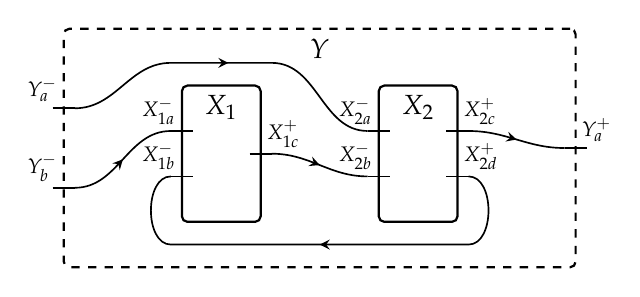
\begin{tikzpicture}[wiring diagram]
  \node[bb={2}{1}, bb name=$X_1$] (X1) {};
  \node[bb={2}{2}, right=of X1, bb name=$X_2$] (X2) {};
  \node[bb={2}{1}, dashed, fit={(X1) (X2) ($(X1.north)+(0,1.5)$) ($(X1.south)-(0,1)$)}, bb name=$Y$] (Y) {};
  \draw[label] 
        node[above left=of Y_in1]     {$Y_a^-$}
        node[above left=of Y_in2]     {$Y_b^-$}
        node[above right=of Y_out1]   {$Y^+_a$}
        node[above left=of X1_in1]    {$X^-_{1a}$}
        node[above left=of X1_in2]    {$X^-_{1b}$}
        node[above right=of X1_out1]  {$X^+_{1c}$}
        node[above left=of X2_in1]    {$X^-_{2a}$}
        node[above left=of X2_in2]    {$X^-_{2b}$}
        node[above right=of X2_out1]  {$X^+_{2c}$}
        node[above right=of X2_out2]  {$X^+_{2d}$};
  \draw[ar] (Y_in2') to (X1_in1);
  \draw[ar] (X1_out1) to (X2_in2);
  \draw[ar] (X2_out1) to (Y_out1');
  \draw[ar] let \p1=(X1.north west), \p2=(X1.north east), \n1={\y1+\bby}, \n2=\bbportlen in
        (Y_in1') to (\x1-\n2,\n1) -- (\x2+\n2,\n1) to (X2_in1);
  \draw[ar] let \p1=(X2.south east), \p2=(X1.south west), \n1={\y1-\bby}, \n2=\bbportlen in
          (X2_out2) to[in=0] (\x1+\n2,\n1) -- (\x2-\n2,\n1) to[out=180] (X1_in2);
\end{tikzpicture}
\end{equation}
represent compositions. That is, new morphisms are constructed from old by specifying which outputs will be fed back into which inputs. In fact, these generalize Penrose diagrams in $\Cat{Vect}$ \todo{true?}\cite{}, and the word \emph{traced} originates in this vector space terminology.  

\section{String diagrams as cobordisms}

A string diagram usually does not explicitly include the outer box $Y$. If we include it, as in (\ref{dia:string diagram}), the resulting \emph{wiring diagram} can be given another interpretation: it represents a 1-dimensional cobordism between oriented 0-manifolds. For example, the box $X_1$ in the picture includes only the data of a pair of finite sets, $(\inp{X_1},\outp{X_1})=(\{1a,1b\},\{1c\})$, which can be interpreted as an oriented 0-manifold.  Moreover, the wiring diagram itself, in which boxes $X_1,\ldots,X_n$ are wired together inside a larger box $Y$, can be interpreted as an oriented cobordism from $X_1\sqcup\cdots\sqcup X_n$ to $Y$. This is a morphism in the multicategory $\Cat{Cob}$, underlying the symmetric monoidal category of oriented 1-cobordisms. \todo[author=Patrick]{Draw this cobordism?}

There is actually a bit more data in a string (or wiring) diagram for a traced category $\cat{C}$. Namely, each input and output of a box must be labeled by an object of $\cat{C}$ and the strings must respect these labels \todo[author=Patrick]{And boxes labeled by morphisms?}. We will thus consider the multicategory $\Cat{Cob}/\cat{O}$ of oriented 1-dimensional cobordisms over a fixed set of labels $\cat{O}$. 

In the table below, we record these two interpretations of a string diagram. Note the ``degree shift'' between the second and third columns.
\begin{center}
% \begin{tabular}{| l | l | l |}
% \hline
% \multicolumn{3}{|c|}{Interpretations of string diagrams}\\\hline
% String diagram & Traced category $\cat{C}$ & $\Cat{Cob}/\cat{O}$\\\bhline
% Wire label set, $\cat{O}$&Objects, $\cat{O}:=\Ob(\cat{C})$&Label set, $\cat{O}$\\
% Box & Morphism & Object (oriented 0-mfd over $\cat{O}$)\\
% String diagram & Composition & Morphism (Cobordism over $\cat{O}$)\\
% Nesting & Axioms of TSMCs & Composition\\\hline
% \end{tabular}
\begin{tabular}{lll}
\toprule
\multicolumn{3}{c}{Interpretations of string diagrams} \\
\midrule
String diagram & Traced category $\cat{C}$ & $\Cat{Cob}/\cat{O}$ \\
\midrule
Wire label set, $\cat{O}$ & Objects, $\cat{O}:=\Ob(\cat{C})$ & Label set, $\cat{O}$ \\
Box \tikz[wiring diagram,bb port sep=1,bby=2.4pt,bb min width=5.5pt,bb port length=2pt,bb rounded corners=1pt,baseline=(B.south)]{\node[bb={1}{2}] (B) {};}
  & Morphism & Object (oriented 0-mfd over $\cat{O}$) \\
String diagram & Composition & Morphism (Cobordism over $\cat{O}$) \\
Nesting & Axioms of TSMCs & Composition \\
\bottomrule
\end{tabular}
\end{center}

The relationship between these interpretations is made precise in the following first main theorem, which will be proved as Corollary~\ref{cor:traced as cob-alg}. For any multicategory $\cat{M}$, we denote by $\cat{M}\alg$ the category of lax functors $\cat{M}\to\Cat{Set}$. Let $\TrCat$ denote the category of traced categories and strong traced functors.

\begin{theorem}\label{thm:traced as cob-alg}
Consider the functor $\op\Set\to\Cat{Cat}$, given by $\cat{O}\mapsto(\Cat{Cob}/\cat{O})\alg$, and let $(\Cat{Cob}/\bullet)\alg$ denote the total category of the corresponding Grothendieck fibration. Then there is an equivalence of categories
$$(\Cat{Cob}/\bullet)\alg\iso\TrCat.$$
\end{theorem}

This will be proved as Corollary~\ref{cor:traced as cob-alg}, but we sketch the equivalence here, with a few minor abuses of notation. It suffices to fix a set $\cat{O}$ and find an equivalence, natural in $\cat{O}$, between the category of $(\Cat{Cob}/\cat{O})$-algebras and the category of traced categories with generating objects $\cat{O}$. We will show that the same data are required, and the same conditions are satisfied, whether one is specifying a lax functor $P\colon\Cat{Cob}/\cat{O}\to\Cat{Set}$ or a traced category $\cat{C}$ with objects generated by $\cat{O}$. 

First, for each box $(\inp{X},\outp{X})$ that might appear in a string diagram, both $P$ and $\cat{C}$ require a set, $P(\inp{X},\outp{X})$ and $\Hom_{\cat{C}}(\inp{X},\outp{X})$, respectively. Second, for each string diagram, both $P$ and $\cat{C}$ require a function: an action on morphisms, in the case of $P$, and a formula for performing the required compositions, tensors, and traces, in the case of $\cat{C}$. The condition that $P$ is functorial corresponds to the fact that $\cat{C}$ satisfies the axioms of traced categories. See Section~\ref{sec:first equivalence} for more pictures that explain the intuition or Section~\ref{**} for the proof.

\section{Generalization: lax algebras on a traced or compact category}

The definition of compact closed symmetric monoidal category, hereafter \emph{compact category}, can be found in Section~\ref{sec:compact and int}, or in \cite{}.

It is most convenient to prove Theorem~\ref{thm:traced as cob-alg} by proving a much more general result, which relates the category of lax functors out of any compact category $\cat{C}$ to the category of strong, bijective-on-objects functors out of $\cat{C}$. Let $\CompCat$ denote the category of compact categories and strong monoidal functors between them. We show in Lemma~\ref{lemma:factorization system} that there is a factorization system on $\CompCat$, in which the left class consists of bijective-on-objects functors and the right class consists of fully faithful functors. Let $\CompCat_{\bo}\ss\CompCat$ denote the left class. 

\begin{theorem}\label{thm:compact lax and strong}
 Let $\cat{C}$ be a compact category. If $\Lax(\cat{C},\Cat{Set})$ denotes the category of lax monoidal set-valued functors out of $\cat{C}$, and $\cat{C}/\CompCat_{\bo}$ denotes the coslice category of compact categories and strong bijective-on-objects functors under $\cat{C}$, then there is an equivalence of categories
\begin{equation}\label{dia:compact lax strong}
  \Lax(\cat{C},\Cat{Set})\cong\cat{C}/\CompCat_{\bo}
\end{equation}
\end{theorem}


Recall from \cite{JoyalStreetVerity} that traced categories are full subcategories of compact categories. The Int construction, applied to a traced category $\cat{C}$, returns the smallest compact category $\Int(\cat{C})$ of which it is a subcategory; we call $\Int(\cat{C})$ the \emph{compact closure} of $\cat{C}$. 

It turns out that if our compact category $\cat{C}$ is the compact closure of a traced category $\cat{D}$, then Theorem~\ref{thm:compact lax and strong} lifts to a result about $\cat{D}$. We record this result as Corollary~\ref{cor:traced lax and strong}, from which Theorem~\ref{thm:traced as cob-alg} follows. 

\begin{corollary}\label{cor:traced lax and strong}
Suppose that $\cat{D}$ is a traced category and its compact closure is $\cat{C}=\Int(\cat{D})$. Then there is an equivalence of categories
\begin{align}\label{dia:traced lax strong}
\Lax(\cat{C},\Cat{Set})\iso\cat{D}/\TrCat_{\bo}
\end{align}
This equivalence is natural in the traced category $\cat{D}$, using the factorization system on $\TrCat$ from Lemma~\ref{lemma:factorization system}.
\end{corollary}

\section{Applications of the operadic perspective}

\subsection{Modular design}

When designing or investigating a complex system, it is often useful to think in terms of interacting subsystems, put together to make a larger whole. In manufacturing, this is often called \emph{modular design}. Each object in $\Cat{Cob}$ represents an interface, or \emph{module}, with a fixed number and type of inputs and outputs. The morphisms in $\Cat{Cob}$ correspond to strategies by which these interfaces can be put together into a process, which itself has an interface. 

An algebra $P\colon\Cat{Cob}\to\Cat{Set}$ provides semantics for these boxes. For each interface $X$, the set $P(X)$ represents the set of ``fillers" for this interface. For example, one might imagine that each interface $X$ can be filled by any state machine having that interface; in this case $P(X)$ is the set of such state machines. For a morphism $\varphi\colon X_1,\ldots,X_n\to Y$, the function $P(\varphi)$ tells us how to construct a filler of type $Y$, given fillers on each $X_i$. Composition of cobordisms are drawn as nested diagrams:

\[
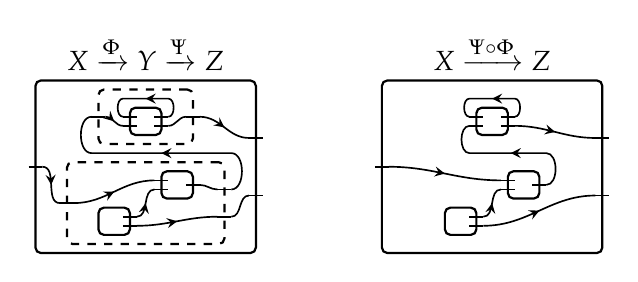
\begin{tikzpicture}[wiring diagram, bb small]
  \node[bb={2}{2}] (X1) {};
  \node[bb={1}{1}, fit={(X1) ($(X1.north)+(0,1)$)}, dashed] (Y1) {};
  \node[bb={2}{1}, below right=4 and 0 of X1] (X2) {};
  \node[bb={0}{2},below left=of X2] (X3) {};
  \node[bb={1}{2}, fit=(X2) (X3), dashed] (Y2) {};
  \node[bb={1}{2}, fit=(Y1) (Y2)] (Z) {};
  \draw[ar] (Z_in1') to (Y2_in1);
  \draw[ar] (Y2_in1') to (X2_in1);
  \draw[ar] (X3_out1) to (X2_in2);
  \draw[ar] (X3_out2) to (Y2_out2');
  \draw (Y2_out2) to (Z_out2');
  \draw[ar] (Y1_in1') to (X1_in2);
  \draw (X1_out2) to (Y1_out1');
  \draw[ar] (Y1_out1) to (Z_out1');
  \draw (X2_out1) to (Y2_out1');
  \draw[ar] let \p1=(Y2.north east), \p2=(Y1.south west), \n1={\y1+\bby}, \n2=\bbportlen in
          (Y2_out1) to[in=0] (\x1+\n2,\n1) -- (\x2-\n2,\n1) to[out=180] (Y1_in1);
  \draw[ar] let \p1=(X1.north east), \p2=(X1.north west), \n1={\y1+\bby}, \n2=\bbportlen in
          (X1_out1) to[in=0] (\x1+\n2,\n1) -- (\x2-\n2,\n1) to[out=180] (X1_in1);
  \node[anchor=south] at (Z.north) {$X\xrightarrow{\Phi}Y\xrightarrow{\Psi}Z$};
  
  \node[bb={2}{2}, right=10 of X1] (X1') {};
  \node[bb={2}{1}, below right=4 and 0 of X1'] (X2') {};
  \node[bb={0}{2},below left=of X2'] (X3') {};
  \node[bb={1}{2}, fit={($(X1'.north)+(0,1)$) (X2') (X3')}, inner xsep=2*\bbx, inner ysep=2*\bby] (Z') {};
  \draw[ar] (X3'_out1) to (X2'_in2);
  \draw[ar] (Z'_in1') to (X2'_in1);
  \draw[ar] (X1'_out2) to (Z'_out1');
  \draw[ar] (X3'_out2) to (Z'_out2');
  \draw[ar] let \p1=(X2'.north east), \p2=(X1'.south west), \n1={\y1+2*\bby}, \n2=\bbportlen in
          (X2'_out1) to[in=0] (\x1+\n2,\n1) -- (\x2-\n2,\n1) to[out=180] (X1'_in2);
  \draw[ar] let \p1=(X1'.north east), \p2=(X1'.north west), \n1={\y1+\bby}, \n2=\bbportlen in
          (X1'_out1) to[in=0] (\x1+\n2,\n1) -- (\x2-\n2,\n1) to[out=180] (X1'_in1);
  \node[anchor=south] at (Z'.north) {$X\xrightarrow{\Psi\circ\Phi}Z$};
\end{tikzpicture}
\]

The story we tell for modular design is that any way to chunk the small boxes inside the big one will give the same result. This is a reflection of the functoriality of $P\colon\Cat{Cob}\to\Set$, which says that commutative diagrams in $\Cat{Cob}$ are sent to commutative diagrams of sets.

\subsection{Mathematical application: varying the operad}

Formalizing modular design using operads, as in \cite{Spivak}, \cite{Rupel-Spivak}, and \cite{Vagner-Spivak-Lerman} was the original motivation for the present paper, as the drawings had strong similarities to those found in traced categories. However, it should be noted that none of these papers actually uses $\Cat{Cob}$ as the indexing category for their algebras. In fact, they use three different operads, of varying degrees of similarity to $\Cat{Cob}$. For example, there is an orthogonal factorization system on $\Cat{Cob}$, for which morphisms in the left class $\cat{L}$ include no closed loops, and \cite{Vagner-Spivak-Lerman} is based on the suboperad spanned by $\cat{L}$.

It is easy to imagine operads with the same objects as $\Cat{Cob}$, but different morphisms, simply by imagining generalizations of the pictures. String diagrams $\varphi\colon X\to Y$ in $\Cat{Cob}$ include no split wires and no ``dangling" wires, but those conditions can be relaxed. Said mathematically, an oriented cobordism $\varphi$ includes the data of a function
$$\varphi_1\colon\inp{X}\sqcup\outp{Y}\to\outp{X}\sqcup\inp{Y},$$
which is both injective and surjective. Either of those conditions can be dropped to generalize the indexing category. 

So while it is difficult to see how to make subtle changes in the axioms of traced categories, it is much more straightforward to see how to make subtle changes in the cobordism operads, which index traced categories.

\section{Plan of the paper}

The paper is organized as follows. In Section~\ref{sec:traced categories} we give more details on the connection between traced monoidal categories, their string diagrams, and algebras on the operad of cobordisms. We conclude that section with a low-tech proof of our main result, Theorem~\ref{thm:traced as cob-alg}, which says that traced categories are $\Cat{Cob}$-algebras. In Section~\ref{sec:generalization} we prove a generalization of that theorem, namely Theorem~\ref{thm:compact lax and strong} and Corollary~\ref{cor:traced lax and strong}, which compare lax set-valued functors to strong bijective-on-objects functors, respectively for compact and traced categories.

\section*{Acknowledgments}

Thanks go to Steve Awodey and Ed Morehouse for suggesting we formally connect our operad-algebra picture to the traced one. 

\chapter{Traced Categories and cobordism algebras}\label{sec:traced categories}

\section{Preliminaries}

Let $\cat{C}$ and $\cat{D}$ be monoidal categories. Recall that a functor $F\colon\cat{C}\to\cat{D}$ is called \emph{lax monoidal} if it is equipped with a morphism
\[
\begin{tikzcd}
	I_D \rar{\epsilon} & F(I_C)
\end{tikzcd}
\]
and a natural transformation
\[
\begin{tikzcd}
	F(X) \otimes_D F(Y) \rar{\mu_{X,Y}} & F(X\otimes_C Y)
\end{tikzcd}
\]
such that for all $X,Y,Z\in\cat{C}$, the diagram (suppressing associators)
\[
\begin{tikzcd}
	F(X)\otimes F(Y) \otimes F(Z)
		\rar{\id\otimes\mu}
		\dar[swap]{\mu\otimes\id}
	& F(X)\otimes F(Y\otimes Z)
		\dar{\mu} \\
	F(X\otimes Y)\otimes F(Z)
		\rar[swap]{\mu}
	& F(X\otimes Y\otimes Z)
\end{tikzcd}
\]
commutes, and for all $X\in\cat{C}$ the two diagrams
\[
\begin{tikzcd}
	I_D\otimes F(X)
		\dar[swap]{\epsilon\otimes\id}
	& F(X)
		\lar[swap]{l_{F(X)}}
		\dar{F(l_X)} \\
	F(I_C)\otimes F(X)
		\rar[swap]{\mu}
	& F(I_C\otimes X)
\end{tikzcd}
\qquad
\begin{tikzcd}
	F(X) \otimes I_D
		\dar[swap]{\id\otimes\epsilon}
	& F(X)
		\lar[swap]{r_{F(X)}}
		\dar{F(r_X)} \\
	F(X)\otimes F(I_C)
		\rar[swap]{\mu}
	& F(X\otimes I_C)
\end{tikzcd}
\]
commute. If $\epsilon$ and $\mu$ are isomorphisms, then $F$ is \emph{strong}.

If $\cat{C}$ and $\cat{D}$ are symmetric monoidal, then $F$ is a \emph{lax symmetric monoidal functor} if it is lax monoidal, and commutes with the symmetries, in the sense that the diagram
\[
\begin{tikzcd}
	F(X)\otimes F(Y)
		\rar{\sigma}
		\dar[swap]{\mu}
	& F(Y)\otimes F(X)
		\dar{\mu} \\
	F(X\otimes Y)
		\rar[swap]{F(\sigma)}
	& F(Y\otimes X)
\end{tikzcd}
\]
commutes.

If $F$ and $G$ are lax monoidal functors (possibly symmetric), then a natural transformation $\alpha\colon F\to G$ is called a \emph{monoidal transformation} if the diagrams
\[
\begin{tikzcd}
	F(X)\otimes F(Y)
		\rar{\alpha_X\otimes\alpha_Y}
		\dar[swap]{\mu}
	& G(X)\otimes G(Y)
		\dar{\mu} \\
	F(X\otimes Y)
		\rar[swap]{\alpha_{X\otimes Y}}
	& G(X\otimes Y)
\end{tikzcd}
\qquad
\begin{tikzcd}[column sep=tiny]
	{} & I_D \dlar[swap]{\epsilon} \drar{\epsilon} & \\
	F(I_C) \ar{rr}[swap]{\alpha_I} && G(I_C)
\end{tikzcd}
\]
commute.

Let $\SymMonCat$ denote the bicategory of symmetric monoidal categories and strong monoidal functors, and let $\Lax(\cat{C},\cat{D})$ denote the category of lax monoidal functors and monoidal transformations from $\cat{C}$ to $\cat{D}$. Let $\CompCat$ denote the full subcategory of $\SymMonCat$ spanned by the compact categories.

% \begin{theorem}
% 	Let $\cat{C}$ be a compact category. There is an equivalence of categories
% 	\[
% 		\Lax(\cat{C},\Set) \simeq (\cat{C}\backslash\CompCat)_{\text{boo}}
% 	\]
% 	between the lax functor category from $\cat{C}$ to $\Set$ equipped with the cartesian monoidal structure, and the full subcategory of the undercategory $\cat{C}\backslash\CompCat$ spanned by the bijective-on-objects functors.
% \end{theorem}
% \begin{proof}
% 	Fix a lax symmetric functor $F\colon\cat{C}\to\Set$. We can construct a compact category $\hat{F}$ and a strong bijective-on-objects functor $\tilde{F}\colon\cat{C}\to\hat{F}$ as follows:
% 	\begin{compactitem}
% 		\item The objects of $\hat{F}$ are the objects of $\cat{C}$.
% 		\item $\Hom_{\hat{F}}(A,B)=F(A^{\star}\otimes B)$.
% 		\item Composition $\Hom(A,B)\times\Hom(B,C)\to\Hom(A,C)$ is defined by
% 		\[
% 		\begin{tikzcd}[column sep=-2ex]
% 			{} & F(A^{\star}\otimes B\otimes B^{\star}\otimes C)
% 				\drar{F(\id\otimes\epsilon_B\otimes\id)} & \\
% 			F(A^{\star}\otimes B)\times F(B^{\star}\otimes C)
% 				\urar{\mu_F}
% 			&& F(A^{\star}\otimes B)
% 		\end{tikzcd}
% 		\]
% 		\item Identities $1\to\Hom(A,A)$ are defined by
% 		\[
% 		\begin{tikzcd}
% 			1 \rar{\epsilon_F} & F(I) \rar{F(\eta_A)} & F(A^{\star}\otimes A).
% 		\end{tikzcd}
% 		\]
% 		\item The tensor product
% 		\[
% 		\begin{tikzcd}
% 			\Hom(A,A')\times\Hom(B,B') \rar{\otimes}
% 			& \Hom(A\otimes B,A'\otimes B')
% 		\end{tikzcd}
% 		\]
% 		is defined by
% 		\[
% 		\begin{tikzcd}[column sep=-3ex]
% 			{} & F(A^{\star}\otimes A'\otimes B^{\star}\otimes B')
% 				\drar{F(\id\otimes\sigma\otimes\id)} & \\
% 			F(A^{\star}\otimes A')\times F(B^{\star}\otimes B')
% 				\urar{\mu_F}
% 			&& F(A^{\star}\otimes B^{\star}\otimes A'\otimes B')
% 		\end{tikzcd}
% 		\]
% 		\item $\tilde{F}$ is identity on objects, and for any $f\colon A\to B$ in $\cat{C}$, define $\tilde{F}(f)$ by
% 		\[
% 		\begin{tikzcd}
% 			1 \rar{\epsilon_F}
% 			& F(I) \rar{F(\eta_A)}
% 			& F(A^{\star}\otimes A) \rar{F(\id\otimes f)}
% 			& F(A^{\star}\otimes B)
% 		\end{tikzcd}
% 		\]
% 		\item The associator and symmetry isomorphisms of $\hat{F}$ are given by the image under $\tilde{F}$ of those in $\cat{C}$.
% 	\end{compactitem}

% 	In the other direction, suppose we are given a compact category $\hat{F}$ and a strong bijective-on-objects functor $\tilde{F}\colon\cat{C}\to\hat{F}$. Define $F$ by
% 	\begin{compactitem}
% 		\item $F(A)=\Hom_{\hat{F}}(I,A)$.
% 		\item For $f\colon A\to B$ in $\cat{C}$, define $F(f)\colon\Hom(I,A)\to\Hom(I,B)$ by post-composition with $\tilde{F}(f)$.
% 		\item $\epsilon\colon 1\to F(I)$ is defined by $\id_I\in\Hom_{\hat{F}}(I,I)$.
% 		\item $\mu\colon F(A)\times F(B)\to F(A\otimes B)$ is defined by
% 		\[
% 		\begin{tikzcd}[column sep=-3ex]
% 			{} & \Hom(I\otimes I,A\otimes B)
% 				\drar & \\
% 			\Hom(I,A)\times\Hom(I,B)
% 				\urar{\otimes_{\hat{F}}}
% 			&& \Hom(I,A\otimes B)
% 		\end{tikzcd}
% 		\]
% 	\end{compactitem}
% \end{proof}


Let $(\cat{M},\otimes,I)$ be a symmetric monoidal category where for any $X,Y\in\Ob(\cat{M})$ we write $\gamma_{X,Y}\colon X\otimes Y\To{\sim} Y\otimes X$ for the distinguished symmetry isomorphisms. Recall that we have $\gamma_{Y,X}=\gamma_{X,Y}^{-1}$.  We define the {\em monoid of scalars in $\cat{M}$} to be the set $S_{\cat{M}}:=\Hom(I,I)$ with multiplication given by composition; in fact $S_{\cat{M}}$ is a commutative monoid.  

There is an action of $S_{\cat{M}}$ on the set $\Hom_{\cat{M}}(X,Y)$ for each $(X,Y)\in\Ob(\cat{M}^{op}\times\cat{M})$, where $s\in S_{\cat{M}}$ acts on a morphism $f\colon X\to Y$ by sending it to the composite morphism
$$s\bullet f\colon X\to I\otimes X\To{s\otimes f}I\otimes Y\to Y.$$
We write $|X|:=\Hom(I,X)$ for the set of \emph{elements} of $X$. The functor $|\cdot|=\Hom(I,\cdot)\colon\cat{M}\to\Set$ is an $\cat{M}$-algebra, i.e., a lax monoidal functor, with unit map
\[\eta\colon\{1\}\To{\id_{I}}\Hom(I,I)\]
and multiplication map
\[\mu\colon\Hom(I,X)\otimes\Hom(I,X')\To{\otimes}\Hom(I\otimes I,X\otimes X')\iso\Hom(I,X\otimes X').\]

\section{Traced categories}\label{sec:intuition for traced}

A trace on a symmetric monoidal category is a collection of functions
\begin{equation}\label{dia:trace function}
\Tr^U_{X,Y}\colon\Hom(U\otimes X,U\otimes Y)\to\Hom(X,Y)
\end{equation}
for $U,X,Y\in\Ob(\cat{M})$ satisfying several axioms. When traced categories are defined, one often sees the trace functions, as well as each of the axioms, accompanied by a picture. For example, (\ref{dia:trace function}) applied to an arbitrary $f\colon U\otimes X\to U\otimes Y$ might be accompanied by this picture:
$$
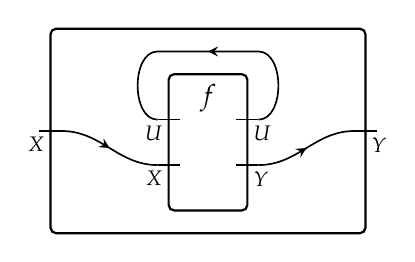
\begin{tikzpicture}[wiring diagram]
  \node[bb={2}{2}, bb name=$f$] (domain) {};
  \node[bb={1}{1}, fit={(domain) ($(domain.north)+(0,1)$)}] (codomain) {};
  \draw[ar] (codomain_in1') to (domain_in2);
  \draw[ar] (domain_out2) to (codomain_out1');
  \draw[ar] let \p1=(domain.north east), \p2=(domain.north west), \n1={\y1+\bby}, \n2=\bbportlen in
          (domain_out1) to[in=0] (\x1+\n2,\n1) -- (\x2-\n2,\n1) to[out=180] (domain_in1);
  \draw[label] 
        node[below left=of codomain_in1]     {$X$}
        node[below right=of codomain_out1]    {$Y$}
        node[below left=of domain_in1]     {$U$}
        node[below left=of domain_in2]     {$X$}
        node[below right=of domain_out2]    {$Y$}
        node[below right=of domain_out1]   {$U$};
 
\end{tikzpicture}
$$
This can be recognized as a cobordism between oriented 0-manifolds, as we will discuss in Section~\ref{sec:Cob morphisms as wds}. Each of the six axioms is vacuous \todo{Is this an appropriate word here?} from this perspective, in that both sides of the equation correspond to the same cobordism. For example, here are the axioms of \emph{dinaturality} and \emph{superposition}:
\begin{itemize}
\item For every $f\colon U\otimes X\to V\otimes Y$ and $g:V\to U$ we have
 \[\Tr^U_{X,Y}\Big[\big(g\otimes Y\big)\circ f\Big]=\Tr^V_{X,Y}\Big[f\circ\big(g\otimes X\big)\Big];\] 
\[\tikzset{bbx=1cm}
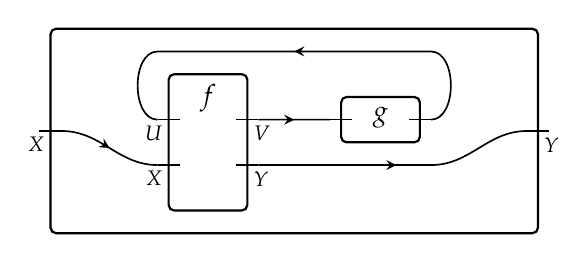
\begin{tikzpicture}[wiring diagram,baseline=(current bounding box.center)] 
  \node[bb={2}{2}, bb name=$f$] (X1) {};
  \node[bb port sep=1,bb={1}{1}, right=.7 of X1_out1, bb name=$g$] (X2) {};
  \node[bb={1}{1}, fit={(X1) (X2) ($(X1.north)+(0,1)$)}] (Y) {};
  \draw[ar] (Y_in1') to (X1_in2);
  \draw[ar,pos=.8] (X1_out1) to (X2_in1);
  \draw[ar] let \p1=(X2.south east), \n1={\y1-\bby}, \n2=\bbportlen in
          (X1_out2) -- (\x1+\n2,\n1) to (Y_out1');
  \draw[ar] let \p1=(X2.north east), \p2=(X1.north west), \n1={\y2+\bby}, \n2=\bbportlen in
          (X2_out1) to[in=0] (\x1+\n2,\n1) -- (\x2-\n2,\n1) to[out=180] (X1_in1);
  \draw[label] 
        node[below left=of Y_in1]     {$X$}
        node[below right=of Y_out1]    {$Y$}
        node[below left=of X1_in1]     {$U$}
        node[below left=of X1_in2]     {$X$}
        node[below right=of X1_out2]    {$Y$}
        node[below right=of X1_out1]   {$V$};
\end{tikzpicture}
=
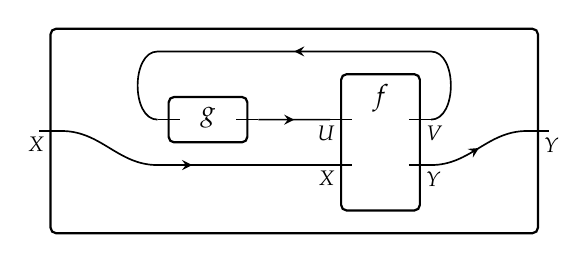
\begin{tikzpicture}[wiring diagram,baseline=(current bounding box.center)] 
  \node[bb={2}{2}, bb name=$f$] (X1) {};
  \node[bb port sep=1,bb={1}{1}, left=.7 of X1_in1, bb name=$g$] (X2) {};
  \node[bb={1}{1}, fit={(X1) (X2) ($(X1.north)+(0,1)$)}] (Y) {};
  \draw[ar] let \p1=(X2.south west), \n1={\y1-\bby}, \n2=\bbportlen in
          (Y_in1') to (\x1-\n2,\n1) -- (X1_in2);
  \draw[ar] (X2_out1) to (X1_in1);
  \draw[ar] (X1_out2) to (Y_out1');
  \draw[ar] let \p1=(X1.north east), \p2=(X2.north west), \n1={\y1+\bby}, \n2=\bbportlen in
          (X1_out1) to[in=0] (\x1+\n2,\n1) -- (\x2-\n2,\n1) to[out=180] (X2_in1);
  \draw[label] 
        node[below left=of Y_in1]     {$X$}
        node[below right=of Y_out1]    {$Y$}
        node[below left=of X1_in1]     {$U$}
        node[below left=of X1_in2]     {$X$}
        node[below right=of X1_out2]    {$Y$}
        node[below right=of X1_out1]   {$V$};
\end{tikzpicture}
\]
\item For every $f\colon U\otimes X\to U\otimes Y$ and $g\colon W\to Z$ we have
 \[\Tr^U_{X,Y}\big[f\big]\otimes g=\Tr^U_{X\otimes W,Y\otimes Z}\big[f\otimes g\big];\]
\[\tikzset{bbx=.8cm,bb port sep=1.5}
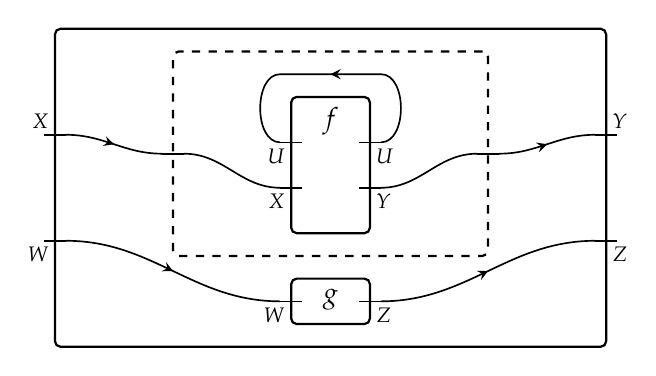
\begin{tikzpicture}[wiring diagram,baseline=(current bounding box.center)] 
  \node[bb={2}{2}, bb name=$f$] (X1) {};
  \node[bb port sep=1,bb={1}{1}, below=2 of X1, bb name=$g$] (X2) {};
  \node[bb={1}{1}, fit={(X1) ($(X1.north)+(0,1)$)}, dashed] (Z) {};
  \node[bb={2}{2}, fit={(Z) (X2)}] (Y) {};
  \draw[ar] (Y_in1') to (Z_in1);
  \draw (Z_in1') to (X1_in2);
  \draw[ar] (Y_in2') to (X2_in1);
  \draw (X1_out2) to (Z_out1');
  \draw[ar] (Z_out1) to (Y_out1');
  \draw[ar] (X2_out1) to (Y_out2');
  \draw[ar] let \p1=(X1.north east), \p2=(X2.north west), \n1={\y1+\bby}, \n2=\bbportlen in
          (X1_out1) to[in=0] (\x1+\n2,\n1) -- (\x2-\n2,\n1) to[out=180] (X1_in1);
  \draw[label] 
        node[above left=of Y_in1] {$X$}
        node[below left=of Y_in2] {$W$}
        node[above right=of Y_out1] {$Y$}
        node[below right=of Y_out2] {$Z$}
        node[below left=of X1_in1] {$U$}
        node[below left=of X1_in2] {$X$}
        node[below right=of X1_out2] {$Y$}
        node[below right=of X1_out1] {$U$}
        node[below left=of X2_in1] {$W$}
        node[below right=of X2_out1] {$Z$};
\end{tikzpicture}
=
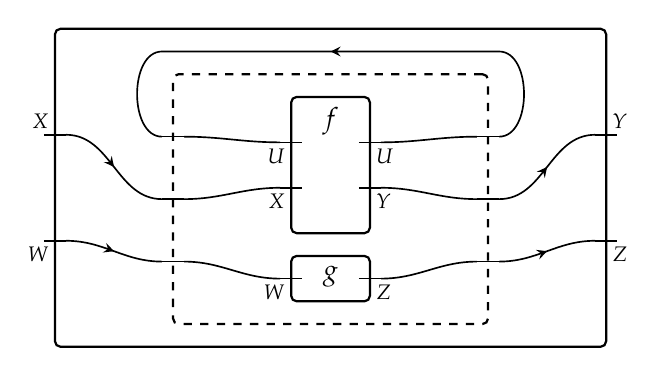
\begin{tikzpicture}[wiring diagram,baseline=(current bounding box.center)] 
  \node[bb={2}{2}, bb name=$f$] (X1) {};
  \node[bb port sep=1,bb={1}{1}, below=of X1, bb name=$g$] (X2) {};
  \node[bb={3}{3}, fit={(X1) (X2)}, dashed] (Z) {};
  \node[bb={2}{2}, fit={(Z) ($(Z.north)+(0,1)$)}] (Y) {};
  \draw[ar] (Y_in1') to (Z_in2);
  \draw (Z_in2') to (X1_in2);
  \draw[ar] (Y_in2') to (Z_in3);
  \draw (Z_in3') to (X2_in1);
  \draw (X1_out2) to (Z_out2');
  \draw[ar] (Z_out2) to (Y_out1');
  \draw (X2_out1) to (Z_out3');
  \draw[ar] (Z_out3) to (Y_out2');
  \draw (Z_in1') to (X1_in1);
  \draw (X1_out1) to (Z_out1');
  \draw[ar] let \p1=(Z.north east), \p2=(Z.north west), \n1={\y1+\bby}, \n2=\bbportlen in
          (Z_out1) to[in=0] (\x1+\n2,\n1) -- (\x2-\n2,\n1) to[out=180] (Z_in1);
  \draw[label] 
        node[above left=of Y_in1] {$X$}
        node[below left=of Y_in2] {$W$}
        node[above right=of Y_out1] {$Y$}
        node[below right=of Y_out2] {$Z$}
        node[below left=of X1_in1] {$U$}
        node[below left=of X1_in2] {$X$}
        node[below right=of X1_out2] {$Y$}
        node[below right=of X1_out1] {$U$}
        node[below left=of X2_in1] {$W$}
        node[below right=of X2_out1] {$Z$};
\end{tikzpicture}
\]
\end{itemize} 

The definition of traced categories and traced functors can be found in \cite{JoyalStreetVerity}.

\erase{%ERASED
\section{Definition of traced category}\label{sec:define traced}

A (left) \emph{trace} on a symmetric monoidal category is a collection of functions 
\[\Tr^U_{X,Y}\colon\Hom(U\otimes X,U\otimes Y)\to\Hom(X,Y)\]
for $U,X,Y\in\Ob(\cat{M})$ satisfying the following axioms:
\begin{description}
 \item [Dinaturality I:] for every $f\colon U\otimes X\to V\otimes Y$ and $g:V\to U$ we have
 \[\Tr^U_{X,Y}\Big[\big(g\otimes Y\big)\circ f\Big]=\Tr^V_{X,Y}\Big[f\circ\big(g\otimes X\big)\Big];\] 
 \item [Naturality:] for every $f\colon U\otimes X\to U\otimes Y$, $g\colon X'\to X$, and $h\colon Y\to Y'$ we have
 \[\Tr^U_{X',Y'}\Big[\big(U\otimes h\big)\circ f\circ\big(U\otimes g\big)\Big]=h\circ\Tr^U_{X,Y}\big[f\big]\circ g;\]
 \item [Superposing:] for every $f\colon U\otimes X\to U\otimes Y$ and $g\colon W\to Z$ we have
 \[\Tr^U_{X,Y}\big[f\big]\otimes g=\Tr^U_{X\otimes W,Y\otimes Z}\big[f\otimes g\big];\]
 \item [Vanishing I:] for every $f\colon X\to Y$ we have
 \[\Tr^{I}_{X,Y}\big[f\big]=f;\]
 \item [Vanishing II:] for every $f\colon U\otimes V\otimes X\to U\otimes V\otimes Y$ we have
 \[\Tr^{U\otimes V}_{X,Y}\big[f\big]=\Tr^V_{X,Y}\Big[\Tr^U_{V\otimes X,V\otimes Y}\big[f\big]\Big];\]
 \item [Yanking:] for any $X\in\Ob(\cat{M})$ we have
 \[\Tr^X_{X,X}\big[\gamma_{X,X}\big]=\id_X.\]
\end{description}
%ERASED
For an object $X$ in a traced category $\cat{M}$ we write $\dim(X):=\Tr^X_{I,I}\big[\id_X\big]\in S_{\cat{M}}$ for the {\em dimension} of $X$.  Note also that for any endomorphism $f\colon X\to X$ there is a scalar $s_f=\Tr^X_{I,I}[f]\in S_{\cat{M}}$.
%ERASED
\begin{proposition}\label{prop:dinaturality}\mbox{}
Let $\cat{M}$ be a symmetric monoidal category.
\begin{enumerate}
 \item If $\cat{M}$ is traced then for every $f\colon X\to Y$ and $g\colon Y\to Z$ in $\cat{M}$, we have
 \[g\circ f=\Tr^Y_{X,Z}\Big[\big(f\otimes g\big)\circ\gamma_{Y,X}\Big].\]
 \item Consider the following axiom:
 \begin{description}
  \item [Dinaturality I':] for every $h\colon U\otimes V\otimes X\to U\otimes V\otimes Y$ we have
 \[\Tr^{U\otimes V}_{X,Y}\big[h\big]=\Tr^{V\otimes U}_{X,Y}\Big[\big(\gamma_{U,V}\otimes Y\big)\circ h\circ\big(\gamma_{V,U}\otimes X\big)\Big].\]
 \end{description}
 In the presence of the other five Axioms, the axioms Dinaturality~I and Dinaturality~I' are equivalent.
\end{enumerate}
\end{proposition}
\begin{proof}
 (1) can be shown from the Naturality and Yanking axioms of the trace as follows:
 \begin{align*}
  \Tr^Y_{X,Z}\Big[\big(f\otimes g\big)\circ\gamma_{Y,X}\Big]
  &=\Tr^Y_{X,Z}\Big[\big(Y\otimes g\big)\circ\big(f\otimes Y\big)\circ\gamma_{Y,X}\Big]\\
  &=\Tr^Y_{X,Z}\Big[\big(Y\otimes g\big)\circ\gamma_{Y,Y}\circ\big(Y\otimes f\big)\Big]\\
  &=g\circ\Tr^Y_{Y,Y}\big[\gamma_{Y,Y}\big]\circ f=g\circ f.
 \end{align*}
 %ERASED
 Dinaturality I' is an immediate consequence of Dinaturality I, indeed apply Dinaturality I with $f=h\circ\big(\gamma_{V,U}\otimes X\big)$ and $g=\gamma_{U,V}$.  For the other direction we apply the composition formula of (1) to the left side of the Dinaturality I equation to get
 \begin{align*}
  \Tr^U_{X,Y}\Big[\big(g\otimes Y\big)\circ f\Big]
  &=\Tr^U_{X,Y}\bigg[\Tr^{V\otimes Y}_{U\otimes X,U\otimes Y}\Big[\big(f\otimes g\otimes Y\big)\circ\gamma_{V\otimes Y,U\otimes X}\Big]\bigg]\\
 &=\Tr^{V\otimes Y\otimes U}_{X,Y}\Big[\big(f\otimes g\otimes Y\big)\circ\gamma_{V\otimes Y,U\otimes X}\Big]\\
  &=\Tr^{V\otimes Y\otimes U}_{X,Y}\Big[\big(f\otimes g\otimes Y\big)\circ\gamma_{V\otimes Y,U\otimes X}\Big]\circ\Tr^X_{X,X}\big[\gamma_{X,X}\big],
 \end{align*}
 where the last two equalities follow from Vanishing II and a trivial application of Yanking.  
 %ERASED
 By Naturality we may bring the first trace into the second to get
 \begin{align*}
  &\Tr^X_{X,Y}\Bigg[\bigg(X\otimes \Tr^{V\otimes Y\otimes U}_{X,Y}\Big[\big(f\otimes g\otimes Y\big)\circ\gamma_{V\otimes Y,U\otimes X}\Big]\bigg)\circ\gamma_{X,X}\Bigg]\\
  &\quad=\Tr^X_{X,Y}\Bigg[\gamma_{Y,X}\circ\bigg(\Tr^{V\otimes Y\otimes U}_{X,Y}\Big[\big(f\otimes g\otimes Y\big)\circ\gamma_{V\otimes Y,U\otimes X}\Big]\otimes X\bigg)\Bigg]\\
  &\quad=\Tr^X_{X,Y}\bigg[\gamma_{Y,X}\circ\Tr^{V\otimes Y\otimes U}_{X\otimes X,Y\otimes X}\Big[\big(f\otimes g\otimes Y\otimes X\big)\circ\big(\gamma_{V\otimes Y,U\otimes X}\otimes X\big)\Big]\bigg]\\
  &\quad=\Tr^X_{X,Y}\bigg[\Tr^{V\otimes Y\otimes U}_{X\otimes X,X\otimes Y}\Big[\big(V\otimes Y\otimes U\otimes \gamma_{Y,X}\big)\circ\big(f\otimes g\otimes Y\otimes X\big)\circ\big(\gamma_{V\otimes Y,U\otimes X}\otimes X\big)\Big]\bigg]\\
  &\quad=\Tr^X_{X,Y}\bigg[\Tr^{V\otimes Y\otimes U}_{X\otimes X,X\otimes Y}\Big[\big(f\otimes g\otimes \gamma_{Y,X}\big)\circ\big(\gamma_{V\otimes Y,U\otimes X}\otimes X\big)\Big]\bigg]\\
  &\quad=\Tr^{V\otimes Y\otimes U\otimes X}_{X,Y}\Big[\big(f\otimes g\otimes \gamma_{Y,X}\big)\circ\big(\gamma_{V\otimes Y,U\otimes X}\otimes X\big)\Big],
 \end{align*}
 where we apply Superposing to get the second equality, Naturality to get the third, and Vanishing II for the last.
 %ERASED
 Now we are ready to apply Dinaturality I' to get
 \begin{align*}
  \Tr^{U\otimes X\otimes V\otimes Y}_{X,Y}\Big[\big(\gamma_{V\otimes Y,U\otimes X}\otimes Y\big)\circ\big(f\otimes g\otimes \gamma_{Y,X}\big)\Big]
 \end{align*}
 from which we may apply, in reverse, an analogous sequence of equalities to that above to get the right hand side of the Dinaturality I equation.
 \erase{\begin{align*}%begin erase
  &=\Tr^Y_{X,Y}\bigg[\Tr^{U\otimes X\otimes V}_{Y\otimes X,Y\otimes Y}\Big[\big(\gamma_{V\otimes Y,U\otimes X}\otimes Y\big)\circ\big(f\otimes g\otimes \gamma_{Y,X}\big)\Big]\bigg]\\
  &=\Tr^Y_{X,Y}\bigg[\Tr^{U\otimes X\otimes V}_{Y\otimes X,Y\otimes Y}\Big[\big(\gamma_{V\otimes Y,U\otimes X}\otimes Y\big)\circ\big(f\otimes g\otimes X\otimes Y\big)\circ\big(U\otimes X\otimes V\otimes \gamma_{Y,X}\big)\Big]\bigg]\\
  &=\Tr^Y_{X,Y}\bigg[\Tr^{U\otimes X\otimes V}_{X\otimes Y,Y\otimes Y}\Big[\big(\gamma_{V\otimes Y,U\otimes X}\otimes Y\big)\circ\big(f\otimes g\otimes X\otimes Y\big)\Big]\circ\gamma_{Y,X}\bigg]\\
  &=\Tr^Y_{X,Y}\Bigg[\bigg(\Tr^{U\otimes X\otimes V}_{X,Y}\Big[\gamma_{V\otimes Y,U\otimes X}\circ\big(f\otimes g\otimes X\big)\Big]\otimes Y\bigg)\circ\gamma_{Y,X}\Bigg]\\
  &=\Tr^Y_{X,Y}\Bigg[\gamma_{Y,Y}\circ\bigg(Y\otimes\Tr^{U\otimes X\otimes V}_{X,Y}\Big[\gamma_{V\otimes Y,U\otimes X}\circ\big(f\otimes g\otimes X\big)\Big]\bigg)\Bigg]\\
  &=\Tr^Y_{Y,Y}\big[\gamma_{Y,Y}\big]\circ\Tr^{U\otimes X\otimes V}_{X,Y}\Big[\gamma_{V\otimes Y,U\otimes X}\circ\big(f\otimes g\otimes X\big)\Big]\\
  &=\Tr^{U\otimes X\otimes V}_{X,Y}\Big[\gamma_{V\otimes Y,U\otimes X}\circ\big(f\otimes g\otimes X\big)\Big]\\
  &=\Tr^{U\otimes X\otimes V}_{X,Y}\Big[\big(g\otimes X\otimes f\big)\circ\gamma_{U\otimes X,V\otimes X}\Big]\\
  &=\Tr^V_{X,Y}\bigg[\Tr^{U\otimes X}_{V\otimes X,V\otimes Y}\Big[\big(g\otimes X\otimes f\big)\circ\gamma_{U\otimes X, V\otimes X}\Big]\bigg]\\
  &=\Tr^V_{X,Y}\Big[f\circ\big(g\otimes X\big)\Big].
 \end{align*}}%end erase
 %%Another proof
 \erase{By Dinaturality I' this becomes%begin erase
 \[\Tr^U_{X,Y}\bigg[\Tr^{Y\otimes V}_{U\otimes X,U\otimes Y}\Big[\big(\gamma_{V,Y}\otimes U\otimes Y\big)\circ\big(f\otimes g\otimes Y\big)\circ\gamma_{V\otimes Y,U\otimes X}\circ\big(\gamma_{Y,V}\otimes U\otimes X\big)\Big]\bigg]\]
 which is equal via Vanishing II and Naturality to
 \begin{align*}
  &\Tr^U_{X,Y}\Bigg[\Tr^V_{U\otimes X,U\otimes Y}\bigg[\Tr^Y_{V\otimes U\otimes X,V\otimes U\otimes Y}\Big[\big(\gamma_{V,Y}\otimes U\otimes Y\big)\circ\big(f\otimes g\otimes Y\big)\circ\gamma_{V\otimes Y,U\otimes X}\circ\big(\gamma_{Y,V}\otimes U\otimes X\big)\Big]\bigg]\Bigg]\\
  &\quad=\Tr^{V\otimes U}_{X,Y}\bigg[\Tr^Y_{V\otimes U\otimes X,V\otimes U\otimes Y}\Big[\big(Y\otimes V\otimes g\otimes Y\big)\circ\big(\gamma_{V,Y}\otimes V\otimes Y\big)\circ\gamma_{V\otimes Y,V\otimes Y}\circ\big(\gamma_{Y,V}\otimes V\otimes Y\big)\circ\big(Y\otimes V\otimes f\big)\Big]\bigg]\\
  &\quad=\Tr^{V\otimes U}_{X,Y}\bigg[\big(V\otimes g\otimes Y\big)\circ\Tr^Y_{V\otimes V\otimes Y,V\otimes V\otimes Y}\Big[\big(\gamma_{V,Y}\otimes V\otimes Y\big)\circ\gamma_{V\otimes Y,V\otimes Y}\circ\big(\gamma_{Y,V}\otimes V\otimes Y\big)\Big]\circ\big(V\otimes f\big)\bigg]\\
  &\quad=\Tr^{V\otimes U}_{X,Y}\bigg[\big(V\otimes g\otimes Y\big)\circ\big(\gamma_{V,V}\otimes Y\big)\circ\big(V\otimes f\big)\bigg].
 \end{align*}
 Applying Dinaturality I' again we get
 \begin{align*}
  &\Tr^{U\otimes V}_{X,Y}\bigg[\big(\gamma_{V,U}\otimes Y\big)\circ\big(V\otimes g\otimes Y\big)\circ\big(\gamma_{V,V}\otimes Y\big)\circ\big(V\otimes f\big)\circ\big(\gamma_{U,V}\otimes X\big)\bigg]\\
  &=\Tr^{U\otimes V}_{X,Y}\bigg[\big(g\otimes f\big)\circ\big(\gamma_{U,V}\otimes X\big)\bigg]\\
  &=\Tr^{U\otimes V}_{X,Y}\bigg[\big(U\otimes f\big)\circ\big(\gamma_{U,U}\otimes X\big)\circ\big(U\otimes g\otimes X\big)\bigg]\\
  &=\Tr^{U\otimes V}_{X,Y}\bigg[\big(U\otimes f\big)\circ\Tr^X_{U\otimes U\otimes X,U\otimes U\otimes X}\Big[\big(\gamma_{U,X}\otimes U\otimes X\big)\circ\gamma_{U\otimes X, U\otimes X}\circ\big(\gamma_{X,U}\otimes U\otimes X\big)\Big]\circ\big(U\otimes g\otimes X\big)\bigg]
 \end{align*}
 Now using Naturality and Vanishing II we get
 \begin{align*}
  &\Tr^{U\otimes V}_{X,Y}\bigg[\Tr^X_{U\otimes V\otimes X,U\otimes V\otimes Y}\Big[\big(X\otimes U\otimes f\big)\circ\big(\gamma_{U,X}\otimes U\otimes X\big)\circ\gamma_{U\otimes X, U\otimes X}\circ\big(\gamma_{X,U}\otimes U\otimes X\big)\circ\big(X\otimes U\otimes g\otimes X\big)\Big]\bigg]\\
  &=\Tr^V_{X,Y}\Bigg[\Tr^U_{V\otimes X,V\otimes Y}\bigg[\Tr^X_{U\otimes V\otimes X,U\otimes V\otimes Y}\Big[\big(\gamma_{U,X}\otimes V\otimes Y\big)\circ\big(g\otimes X\otimes f\big)\circ\gamma_{U\otimes X, V\otimes X}\circ\big(\gamma_{X,U}\otimes V\otimes X\big)\Big]\bigg]\Bigg]\\
  &=\Tr^V_{X,Y}\bigg[\Tr^{X\otimes U}_{V\otimes X,V\otimes Y}\Big[\big(\gamma_{U,X}\otimes V\otimes Y\big)\circ\big(g\otimes X\otimes f\big)\circ\gamma_{U\otimes X, V\otimes X}\circ\big(\gamma_{X,U}\otimes V\otimes X\big)\Big]\bigg]
 \end{align*}
 which by Dinaturality I' is equal to
 \[\Tr^V_{X,Y}\bigg[\Tr^{U\otimes X}_{V\otimes X,V\otimes Y}\Big[\big(g\otimes X\otimes f\big)\circ\gamma_{U\otimes X, V\otimes X}\Big]\bigg],\]
 but this is exactly the composition formula applied to the right hand side of Dinaturality I.}%end erase
\end{proof}
%ERASED
\begin{definition}\label{def:traced functor}

Let $(\cat{M},\otimes,\tensor*[^{\cat{M}}]{\Tr}{})$ and $(\cat{N},\odot,\tensor*[^{\cat{N}}]{\Tr}{})$ be traced categories. A \emph{traced functor} is a strong monoidal functor $F\colon\cat{M}\to\cat{N}$, such that for any objects $X,Y,U\in\cat{M}$, the following diagram commutes:
$$
\begin{tikzcd}
	\Hom_{\cat{M}}(U\otimes X,U\otimes Y)
		\rar{F}
		\dar[swap]{\tensor*[^{\cat{M}}]{\Tr}{^U_{X,Y}}}
	& \Hom_{\cat{N}}(FU\odot FX,FU\odot FY)
		\dar{\tensor*[^{\cat{N}}]{\Tr}{^{FU}_{FX,FY}}} \\
	\Hom_{\cat{M}}(X,Y)
		\rar[swap]{F}
	& \Hom_{\cat{N}}(FX,FY)
\end{tikzcd}
$$
We generally suppress the upper left subscripts from the trace symbols, if no confusion is likely to arise.

\end{definition}

}%ERASED

\section{Compact categories and the Int construction}\label{sec:compact and int}

Let $\SymMonCat$ denote the category of symmetric monoidal functors and strong morphisms between them. We will denote by $\CompCat\ss\SymMonCat$ the full subcategory spanned by compact categories. Recall that a compact category is a symmetric monoidal category $(\cat{C},\otimes,I)$ with the property that for every object $X\in\Ob\cat{C}$ there exists an object $X^*$ and morphisms $\eta_X\colon I\to X^*\otimes X$ and $\epsilon_X\colon X\otimes X^*\to I$ such that the following diagrams commute:
$$\begin{tikzcd}[column sep=small]
X\arrow[r,"\id_X"]\arrow[d,"\cong"']&X\\
X\otimes I\arrow[d,"X\otimes\eta_X"']&I\otimes X\arrow[u,"\cong"']\\
X\otimes(X^*\otimes X)\arrow[r,"\cong"']&(X\otimes X^*)\otimes X\arrow[u,"\epsilon_X\otimes X"']
\end{tikzcd}
\hspace{.6in}
\begin{tikzcd}[column sep=small]
X^*\arrow[r,"\id_{X^*}"]\arrow[d,"\cong"']&X^*\\
I\otimes X^*\arrow[d,"\eta_X\otimes X^*"']&X^*\otimes I\arrow[u,"\cong"']\\
(X^*\otimes X)\otimes X^*\arrow[r,"\cong"']&X^*\otimes (X\otimes X^*)\arrow[u,"X^*\otimes\epsilon_X"']
\end{tikzcd}
$$

Every compact category $\cat{C}$ has a canonical trace structure, defined on a morphism $f\colon U\otimes X\to U\otimes Y$ to morally be $\epsilon_U\circ f\circ \eta_U$. More precisely, if $s_{A,B}$ is the symmetry isomorphism, one defines
$$\Tr^U_{X,Y}[f]:=(\epsilon_U\otimes Y)\circ (s_{U^*,U}\otimes Y)\circ (U^*\otimes f)\circ (\eta_U\otimes X)$$
%\todo[color=yellow]{does this formula make sense as written? i.e. it doesn't seem to give a map $X\to Y$?} 
Thus we have a functor 
$U\colon\CompCat\to\TrCat$. It is shown in \cite{Joyal-Street-Verity} that this functor is the right half of an adjunction 
\begin{equation}\label{dia:traced compact adjunction}
\begin{tikzcd}
\TrCat\arrow[r,shift left=.5ex, "\Int"]&\CompCat\arrow[l,shift left=.5ex,"U"]
\end{tikzcd}
\end{equation}
the left half of which we describe now describe. 

For a traced category $\cat{M}$ let $\widetilde{\cat{M}}=\Int(\cat{M})$ denote the category with objects given by pairs $(\inp{X},\outp{X})$ where $\inp{X},\outp{X}\in \Ob(\cat{M})$ and morphisms given by 
\[\Hom_{\widetilde{\cat{M}}}\big((\inp{X},\outp{X}),(\inp{Y},\outp{Y})\big)=\Hom_{\cat{M}}(\inp{X}\otimes \outp{Y},\outp{X}\otimes \inp{Y}).\]
For morphisms $\Phi:(\inp{X},\outp{X})\to(\inp{Y},\outp{Y})$ and $\Psi:(\inp{Y},\outp{Y})\to(\inp{Z},\outp{Z})$ in $\widetilde{\cat{M}}$ we define their composition to be
\[\Psi\circ\Phi:=\Tr^{\outp{Y}}_{\inp{X}\otimes \outp{Z},\outp{X}\otimes \inp{Z}}\Big[\big(\gamma_{\outp{X},\outp{Y}}\otimes \inp{Z}\big)\circ\big(\outp{X}\otimes\Psi\big)\circ\big(\Phi\otimes \outp{Z}\big)\circ\big(\gamma_{\outp{Y},\inp{X}}\otimes \outp{Z}\big)\Big].\]
It is shown in \cite{JoyalStreetVerity} that $\widetilde{\cat{M}}$ is a compact  category whose tensor is given by
\[(\inp{X},\outp{X})\odot(\inp{Y},\outp{Y}):=(\inp{X}\otimes \inp{Y},\outp{X}\otimes \outp{Y})\]
with unit object $\tilde I:=(I,I)$ and duality $(\inp{X},\outp{X})^\vee:=(\outp{X},\inp{X})$.  The following is immediate from the definitions.

\begin{lemma}\todo{This lemma has a sign-error. Either change definition of $\Hom_{\widetilde{\cat{M}}}$ or lemma statement.}

Let $\cat{M}$ be a traced category.  Then for any object $(\inp{X},\outp{X})\in\Ob\big(\widetilde{\cat{M}}\big)$ there is a canonical bijection
\[|(\inp{X},\outp{X})|\iso\Hom_{\cat{M}}(\inp{X},\outp{X}).\]

\end{lemma}

\todo{Perhaps we should explain somewhere how the adjunction works, and update the proof of Lemma~\ref{lemma:more fully faithfulness} if necessary.}

\begin{lemma}\label{lemma:fully faithful and trace}
The following facts hold for any traced category $\cat{C}$:
\begin{compactitem}
	\item The unit $\cat{C}\to\Int(\cat{C})$ is fully faithful.
	\item If $\cat{D}$ is a category and $F\colon\cat{D}\to\cat{C}$ a fully faithful symmetric monoidal functor, then $\cat{D}$ has a unique trace for which $F$ is a traced functor.
\end{compactitem}
\end{lemma}

\begin{proof}

These are all shown in \cite{Joyal-Street-Verity}.

\end{proof}

\section{Free Constructions}

To continue we recall the constructions of various free monoidal structures on a category $\cat{C}$ following \cite{abramsky}.  These are defined inductively by successively including additional structure into the constructions.

The objects of the free monoidal category $F_M(\cat{C})$ are lists of objects in $\cat{C}$ with componentwise morphisms.  More formally the objects are pairs $(n,X)$ where $n\in\NN$ and $X$ is a map $X\colon[n]\to \Ob\cat{C}$ and a morphism $f:(n,X)\to(m,Y)$ exists if and only if $n=m$ in which case $f\in\prod_{i=1}^n\Hom_{\cat{C}}(X_i,Y_i)$ with compositions formed as expected.  The tensor product is given by concatenation of lists, i.e. $(n,X)\otimes(m,Y)=(n+m,X+Y)$, with tensor unit $(0,!)$ where $!$ is the unique function from the empty set.

The objects of the free symmetric monoidal category $F_{SM}(\cat{C})$ are again lists of objects in $\cat{C}$, however morphisms now come equipped with a permutation.  More formally, a morphism from $(n,X)$ to $(n,Y)$ is a pair $(f,\pi)$ where $f\in\prod_{i=1}^n\Hom_{\cat{C}}(X_i,Y_{\pi(i)})$ and $\pi\in S(n)$ is a permutation.  By abuse of notation a permutation can be thought of as an isomorphism $\pi:Y_1\otimes\cdots\otimes Y_n\To{\sim} Y_{\pi(1)}\otimes\cdots\otimes Y_{\pi(n)}$ and thus we may think of the pair $(f,\pi)$ as the composite 
\[\pi^{-1}\circ \bigotimes_{i=1}^n f_i:\bigotimes_{i=1}^n X_i\to\bigotimes_{i=1}^n Y_i.\]
The symmetry isomorphisms are subject to the naturality condition $\otimes_{i=1}^n g_{\pi(i)}\circ\pi=\pi\circ\otimes_{i=1}^n g_i$ for functions $g_i:Y_i\to Z_i$.  Then the composition of morphisms is given by 
$$(g,\sigma)\circ(f,\pi):=\Big(\bigotimes_{i=1}^n (g_{\pi(i)}\circ f_i),\sigma\circ\pi\Big)$$ 
and the tensor is given by 
$$(f,\pi)\otimes(g,\sigma):=(f\otimes g,\pi\otimes\sigma).$$

The objects of the free traced symmetric monoidal category $F_{Tr}(\cat{C})$ are once again lists of objects in $\cat{C}$.  To describe the morphisms we need more notation.  Write $L[\cat{C}]$ for the set of \emph{loops} of $\cat{C}$, i.e. the set of all composable sequences of morphisms $A_1\To{f_1} A_2\To{f_2}\cdots\To{f_{m-1}} A_m\To{f_m} A_1$ in $\cat{C}$.  Because we are in the traced setting each such sequence $f$ determines a scalar $s_f:=\Tr_{I,I}^{A_1}[f_m\circ\cdots\circ f_1]$ which is invariant under cyclic permutation of the morphisms, thus we only consider loops in $\cat{C}$ up to cyclic rotation.  Now a morphism in $F_{Tr}(\cat{C})$ is a triple $(f,\pi,S)$ where $(f,\pi)$ is a morphism in $F_{SM}(\cat{C})$ and $S$ is an element of the free commutative monoid generated by $L[\cat{C}]$.  The composition and tensor of morphisms are given by
\[(g,\sigma,T)\circ(f,\pi,S)=\Big(\bigotimes_{i=1}^n (g_{\pi(i)}\circ f_i),\sigma\circ\pi,S\cdot T\Big)\]
and
\[(f,\pi,S)\otimes(g,\sigma,T)=(f\otimes g,\pi\otimes\sigma,S\cdot T).\]
The trace requires yet more notation.  For a permutation $\pi\in S(n+m)$ and $1\le i\le n$ write $P_\pi(i)$ for the unique sequence $i,\pi(i),\pi^2(i),\ldots,\pi^r(i)=j$ such that $1\le j\le n$ and $\pi^t(i)>n$ for $0<t<r$, in this case we write $\pi^*(i)=j$.  Thus we may obtain a permutation $\pi^*\in S(n)$ by removing all occurences of $\{n+1,\ldots,n+m\}$ from a cycle decomposition of $\pi$.  This process may produce empty cycles which we will want to keep track of.  Write $L_\pi$ for the collection of loops of $\pi$, i.e. sequences $j,\pi(j),\pi^2(j),\ldots,\pi^s(j)=j$ (taken up to cyclic symmetry) such that $n+1\le \pi^t(j)\le n+m$ for $0\le t\le s$.  Now we define the trace of a morphism $(f,\pi,S)$ as
\[\Tr_{n,n}^m[(f,\pi,S)]=(g,\pi^*,S\cdot T)\]
where $g_i=f_{\pi^r(i)}\circ\cdots\circ f_{\pi(i)}\circ f_i$ and $T=\prod\limits_{j\in L_\pi} \Tr_{I,I}^{X_j}[f_{\pi^s(j)}\circ\cdots f_{\pi(j)}\circ f_j]$.

By \cite{Abramsky}, $\Cat{Cob}/\cat{O}$ is the free compact category on the set $\cat{O}$ of objects. The objects in $\Cat{Cob}/\cat{O}$ are signed symmetric lists in $\cat{O}$, the set of which we denote by $\Ob(\Cat{Cob}/\cat{O})=\SSList(\cat{O})$. Theorem~\ref{thm:compact lax and strong} amounts to the following equivalence of categories, when $\cat{C}=\Cat{Cob}/\cat{O}$:\todo{This and the following remark probably don't go here.}
$$\Lax(\Cat{Cob}/\cat{O},\Cat{Set})\iso\CompCat_{\boo\SSList(\cat{O})}.$$

\begin{remark}

Let $\cat{V}$ denote a symmetric monoidal category. To the best of our knowledge, neither the category of $\cat{V}$-enriched compact categories nor the category of $\cat{V}$-enriched traced categories has been defined in the literature. Theorem~\ref{thm:compact lax and strong} and Corollary~\ref{cor:traced lax and strong} could be used to motivate a definition of these categories by replacing $\Cat{Set}$ with $\cat{V}$ in (\ref{dia:compact lax strong}) and (\ref{dia:traced lax strong}). That is, one could define a $\cat{V}$-enriched compact category to be a set $\cat{O}$ and a lax functor $\Cat{Cob}/\cat{O}\to\cat{V}$. 

It is worth exploring whether this definition agrees with other possible or existing definitions of enriched traced categories and enriched compact categories.

\end{remark}



\section{Wiring Diagrams and $\Cat{Cob}$}\label{sec:wds and cob}

In this section, we more carefully explain the equivalence between the category of traced categories and the category of cobordism algebras.

\subsection{Objects in $\Cat{Cob}$ as interfaces}

The objects in $\Cat{Cob}$ are signed sets $(\inp{X},\outp{X})$, each of which can be drawn as a box with input wires $\inp{X}$ drawn entering the box, on its left, and output wires $\outp{X}$ drawn exiting the box, on its right. We call the latter style \emph{an interface}.

\begin{figure}
\[
\begin{tikzpicture}[node distance=0 and 0, baseline=(current bounding box.center)]
  \node (A1) {$-$};
  \node[below=of A1] (A2) {$-$};
  \node[below=of A2] (A3) {$-$};
  \node[below=of A3] (B1) {$+$};
  \node[below=of B1] (B2) {$+$};
\end{tikzpicture}
\hspace{4em}
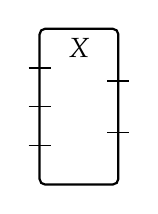
\begin{tikzpicture}[wiring diagram, bby=1.5ex, baseline=(current bounding box.center)]
  \node[bb={3}{2},bb name=$X$] {};
\end{tikzpicture}
\]
\caption{The signed set $(\ul{3},\ul{2})$, drawn in the usual style and as an interface.}
\end{figure}

\subsection{Morphisms in $\Cat{Cob}$ as wiring diagrams}\label{sec:Cob morphisms as wds}

Wiring diagrams seem to be a new way to visualize morphisms in the symmetric monoidal category $\Cat{Cob}$ of 1-dimensional oriented cobordisms.

\[
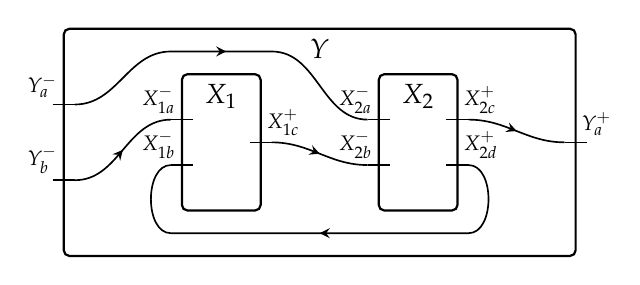
\begin{tikzpicture}[wiring diagram, baseline=(current bounding box.center)]
  \node[bb={2}{1}, bb name=$X_1$] (X1) {};
  \node[bb={2}{2}, right=of X1, bb name=$X_2$] (X2) {};
  \node[bb={2}{1}, fit={(X1) (X2) ($(X1.north)+(0,1)$) ($(X1.south)-(0,1)$)},bb name =$Y$] (Y) {};
  \draw[label] 
        node[above left=of Y_in1]     {$\inp{Y}_a$}
        node[above left=of Y_in2]     {$\inp{Y}_b$}
        node[above right=of Y_out1]   {$\outp{Y}_a$}
        node[above left=of X1_in1]    {$\inp{X}_{1a}$}
        node[above left=of X1_in2]    {$\inp{X}_{1b}$}
        node[above right=of X1_out1]  {$\outp{X}_{1c}$}
        node[above left=2pt and -2pt of X2_in1]    {$\inp{X}_{2a}$}
        node[above left=of X2_in2]    {$\inp{X}_{2b}$}
        node[above right=of X2_out1]  {$\outp{X}_{2c}$}
        node[above right=of X2_out2]  {$\outp{X}_{2d}$};
  \draw[ar] (Y_in2') to (X1_in1);
  \draw[ar] (X1_out1) to (X2_in2);
  \draw[ar] (X2_out1) to (Y_out1');
  \draw[ar] let \p1=(X1.north west), \p2=(X1.north east), \n1={\y1+\bby}, \n2=\bbportlen in
        (Y_in1') to (\x1-\n2,\n1) -- (\x2+\n2,\n1) to (X2_in1);
  \draw[ar] let \p1=(X2.south east), \p2=(X1.south west), \n1={\y1-\bby}, \n2=\bbportlen in
          (X2_out2) to[in=0] (\x1+\n2,\n1) -- (\x2-\n2,\n1) to[out=180] (X1_in2);
\end{tikzpicture}
\qquad
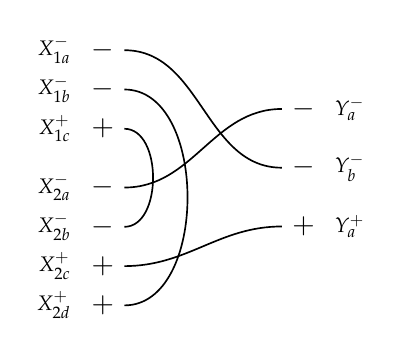
\begin{tikzpicture}[x=1cm,y=1ex,node distance=1 and 1,semithick,every label quotes/.style={font=\everymath\expandafter{\the\everymath\scriptstyle}},every to/.style={out=0,in=180},baseline=(current bounding box.center)]
  \node ["$\inp{X}_{1a}$" left] (X1a) {$-$};
  \node [below=0 of X1a, "$\inp{X}_{1b}$" left] (X1b) {$-$};
  \node [below=0 of X1b, "$\outp{X}_{1c}$" left] (X1c) {$+$};
  \node [below=1.5 of X1c, "$\inp{X}_{2a}$" left] (X2a) {$-$};
  \node [below=0 of X2a, "$\inp{X}_{2b}$" left] (X2b) {$-$};
  \node [below=0 of X2b, "$\outp{X}_{2c}$" left] (X2c) {$+$};
  \node [below=0 of X2c, "$\outp{X}_{2d}$" left] (X2d) {$+$};
  \node [below right=1.5 and 2 of X1a, "$\inp{Y}_a$" right] (Ya) {$-$};
  \node [below=1.5 of Ya, "$\inp{Y}_b$" right] (Yb) {$-$};
  \node [below=1.5 of Yb, "$\outp{Y}_a$" right] (Yc) {$+$};
  \draw (X1a) to (Yb);
  \draw (X1b) to[in=0] (X2d);
  \draw (X1c) to[in=0] (X2b);
  \draw (X2a) to (Ya);
  \draw (X2c) to (Yc);
\end{tikzpicture}
\]



\subsection{The $\Cat{Cob}$-algebra perspective: building nested structures}

For a fixed set $\cat{O}$, a $\Cat{Cob}/\cat{O}$-algebra is a lax functor $I\colon\Cat{Cob}/\cat{O}\to\Set$. In this perspective, each box $X\in\Cat{Cob}/\cat{O}$ is an interface, and $I(X)$ is the set of \emph{inhabitants} that conform to that interface. A morphism $\varphi\colon X_1,\ldots,X_n\to Y$ in $\Cat{Cob}/\cat{O}$ is a wiring-together of interfaces, and if an inhabitant is given for each of the $X_i$, the algebra $I$ gives a formula for producing an inhabitant of $Y$. Nested structures, given by composition of such morphisms, may be useful for the kind of chunking that humans use to understand complex systems. \cite{Miller, George A. "The magical number seven, plus or minus two: some limits on our capacity for processing information." Psychological review 63.2 (1956): 81.}

\section{A factorization system for strong functors}

In this section we prove that an orthogonal factorization system exists on the categories $\SymMonCat$, $\TrCat$, and $\CompCat$ of symmetric monoidal (resp. traced, compact) categories and strong functors (resp. traced functors; see Definition~\ref{def:traced functor}). 

Recall from \cite{} that an \emph{orthogonal factorization system} on a category $\cat{C}$ consists of a class $\cat{L}$ and a class $\cat{R}$ of morphisms in $\cat{C}$, called the \emph{left class} and \emph{right class} of the factorization system, respectively, satisfying the following properties:
\begin{enumerate}
\item $\cat{L}$ (resp. $\cat{R}$) contains every isomorphism in $\cat{C}$, 
\item $\cat{L}$ (resp. $\cat{R}$) is closed under composition, and
\item every morphism $f\in\cat{C}$ can be uniquely and functorially factored as $f=r\circ\ell$ where $r\in\cat{R}$ and $\ell\in\cat{L}$
\end{enumerate}
For example, there is an orthogonal factorization system on $\Cat{Cat}$ in which the left class consists of functors that are bijective on objects and the right class consists of functors that are fully faithful. 



\begin{lemma}\label{lemma:factorization system}

Let $\XCat$ denote the category of strong $\Cat{X}$-functors between $\Cat{X}$-categories,  where $\Cat{X}$ is plain, monoidal, traced, or compact. Then $\XCat$ admits an orthogonal factorization system $(\cat{L},\cat{R})$, where the morphisms in $\cat{L}$ are bijective-on-objects functors and the morphisms in $\cat{R}$ are fully faithful functors.

\end{lemma}

\begin{proof}

We first recall the factorization system $(\bo,\ff)$ on $\Cat{Cat}$. Let $\cat{C}$ and $\cat{D}$ be categories, and let $F\colon\cat{C}\to\cat{D}$ be a functor. Then there is a factorization
\[
\begin{tikzcd}[column sep=small, row sep=small]
  \cat{C} \ar[rr, "F"] \ar[dr, "\bo"'] && \cat{D} \\
  & \cat{F} \ar[ur, "\ff"']
\end{tikzcd}
\]
where $\cat{F}$ is the category with $\Ob\cat{F}:=\Ob\cat{C}$, $\Hom_{\cat{F}}(c_1,c_2):=\Hom_{\cat{D}}(Fc_1,Fc_2)$, and composition defined by composition in $\cat{D}$. The ``bo'' functor is the identity on objects, and $F$ on morphisms, while the ``ff'' functor is $F$ on objects and the identity on morphisms.

Note that to establish the factorization system for $\XCat$, the only thing that needs to be checked is that the factorization in $\Cat{Cat}$ lifts to $\XCat$. The isomorphism containment, closure under composition, and uniqueness of factorization all follow immediately from those same properties in $\Cat{Cat}$.

Now we will show that this factorization system lifts to $\MonCat$. If $\cat{C}$ and $\cat{D}$ are monoidal categories, and $F$ is a strong monoidal functor, then we can define a monoidal structure on $\cat{F}$. On objects, define $c_1\otimes_{\cat{F}}c_2:=c_1\otimes_{\cat{C}}c_2$ with monoidal unit $I_{\cat{F}}:=I_{\cat{C}}$, and given morphisms $f_1\colon c_1\to c_1'$ and $f_2\colon c_2\to c_2'$ in $\cat{F}$, i.e.~morphisms $f_1\colon Fc_1\to Fc_1'$ and $f_2\colon Fc_2\to Fc_2'$ in $\cat{D}$, define $f_1\otimes_{\cat{F}}f_2$ to be the composition
\[
\begin{tikzcd}
  F(c_1\otimes_{\cat{C}}c_2) \ar[r,"\mu^{-1}"] & F(c_1)\otimes_{\cat{D}}F(c_2) \ar[r,"f_1\otimes_{\cat{D}}f_2"] & F(c_1')\otimes_{\cat{D}}F(c_2') \ar[r,"\mu"] & F(c_1'\otimes_{\cat{C}}c_2').
\end{tikzcd}
\]
The coherence isomorphisms of $\cat{F}$ are defined by applying $F$ to the coherence isomorphisms of $\cat{C}$, e.g.~the left unitor $l_{\cat{F}}\colon c\to I_{\cat{C}}\otimes_{\cat{C}}c$ is defined to be $F(l_{\cat{C}})\colon F(c)\to F(I_{\cat{C}}\otimes_{\cat{C}}c)$. The monoidal category axioms can then be checked for $\cat{F}$ using the fact that $F$ is strong monoidal. Finally, the ``bo'' functor is trivialy strict monoidal, and the ``ff'' functor has a strong monoidal structure using the same coherence isomorphsisms as $F$.

Suppose that $\cat{C}$ and $\cat{D}$ are both compact categories. Every object of $\cat{F}$ is the image of an object in $\cat{C}$, and every object of $\cat{C}$ has a dual, hence every object of $\cat{F}$ has a dual because monoidal functors always preserve duals. This shows that the (bo,ff) factorization system lifts to $\CompCat$.

Finally, if $\Cat{C}$ and $\cat{D}$ are traced, then \cite[Proposition 2.4]{Joyal-Street-Vertity} implies that there is a unique traced structure on $\cat{F}$, where the trace of a morphism in $\cat{F}$ is defined to be the trace in $\cat{D}$. The ``ff'' functor preserves the trace by construction, and the ``bo'' functor preserves the trace because $F$ does.
\end{proof}

\begin{proposition}
  There is a contravariant functor $\XCat\to\Cat{Cat}$ sending any $\cat{C}\in\XCat$ to the category $\cat{C}/\XCat_{\bo}$.
\end{proposition}
\begin{proof}
  We only need to verify the functoriality of this construction. Given a strong functor $F\colon\cat{C}\to\cat{D}$ in $\XCat$, we can define a functor $F^*\colon\cat{D}/\XCat_{\bo}\to\cat{C}/\XCat_{\bo}$. For any object $\phi\in\cat{D}/\XCat_{\bo}$, i.e.~ a bijective-on-objects functor $\phi\colon\cat{D}\to\cat{X}$, define $F^*(\phi)$ by applying the factorization system of \ref{lemma:factorization system} as in the diagram
  \[
  \begin{tikzcd}
    \cat{C} \ar[r,"F"] \ar[d,"F^*(\phi)"'] & \cat{D} \ar[d,"\phi"] \\
    \cat{X}' \ar[r,"\ff"'] & \cat{X}
  \end{tikzcd}
  \]
\end{proof}

\begin{proposition}\label{prop:free objects}

Let $\XCat$ denote the category of strong $\Cat{X}$-functors between $\Cat{X}$-categories,  where $\Cat{X}$ is monoidal, traced, or compact, and let $\Cat{XFrObCat}$ denote the full subcategory spanned by strict, free-on-objects $\Cat{X}$-categories, i.e., for which the symmetric monoid of objects is free. There is an adjoint 2-equivalence:
$$
\begin{tikzcd}
\XCat\arrow[r, shift left=.5ex, "\Fun{FrOb}"]&\Cat{XFrObCat}\arrow[l, shift left=.5ex,"U"]
\end{tikzcd}
$$
where $U$ is the forgetful inclusion. In particular, for every $\Cat{X}$-category $\cat{C}$ there is a strict $\Cat{X}$-category $\Fun{FrOb}(\cat{C})$, whose symmetric monoid of objects is free, and an equivalence in $\XCat$:
$$\Fun{FrOb}(\cat{C})\simeq\cat{C}.$$

\end{proposition}

\begin{proof}

\cite{Abramsky} provides a free-forgetful adjunction
$$
\begin{tikzcd}
\Cat{Cat}\arrow[r, shift left=.5ex, "F"]&\XCat\arrow[l, shift left=.5ex,"G"]
\end{tikzcd}
$$
For any $\Cat{X}$-category $\cat{C}$, we have a counit $FG(\cat{C})\to\cat{C}$, which is surjective on objects. We define $\Fun{FrOb}(\cat{C})$ to be the factorizing object for the factorization system from Lemma~\ref{lemma:factorization system}:
$$
\begin{tikzcd}[column sep=small]
FG(\cat{C})\arrow[dr, "bo"']\arrow[rr, "F"]&&\cat{C}\\
&\Fun{FrOb}(\cat{C})\arrow[ur, "ff"']
\end{tikzcd}
$$
The right-hand functor is fully faithful and clearly surjective, so it is an equivalence of categories. This proves that $\Fun{FrOb}\circ\fun{U}\iso\id$, and because $U$ is a monomorphism, we have $U\circ\Fun{FrOb}\iso\id$ as well.

\todo{This has not been checked.}

\end{proof}

\section{The equivalence $\TrCat\simeq(\Cat{Cob}/\bullet)\alg$}\label{sec:first equivalence}

\todo{The point of this proof is not to be rigorous, because we already prove this elsewhere. The point is to give better intuition for the result. Rewrite with that in mind. Use more pictures.}

\begin{theorem}\label{thm:cob-O and traced-O}
For any set $\cat{O}$, let $\SList(\cat{O})$ denote the set of symmetric lists in $\cat{O}$. There is an equivalence of categories 
 $$(\Cat{Cob}/\cat{O})\alg\simeq\TrCat_{\boo\SList(\cat{O})}$$
\end{theorem}
\begin{proof}
 Dylan....\\
\todo[author=Patrick]{I think this only needs to be a proof sketch} 
 \bigskip

 Let $\cat{M}$ be a traced category with objects $\SList(\cat{O})$. We will define a $\Cat{Cob}/\cat{O}$-algebra $\cat{P}=R(\cat{M})\colon\Cat{Cob}/\cat{O}\to\Cat{Set}$ as follows. For an object $X\in\Ob(\Cat{Cob}/\cat{O})$, set 
$$\cat{P}(X):=\Hom_{\cat{M}}(\vinp{X},\voutp{X}).$$
We next consider morphisms.

Following Proposition~\ref{prop:set theoretic cob1} (borrow notation/setup from Abramsky instead) a morphism $\Phi\colon X\longrightarrow Y$ consists of a typed bijection 
$$\varphi\colon\inp{X}\sqcup \outp{Y}\xrightarrow{\iso}\outp{X}\sqcup \inp{Y},$$ 
together with a typed finite set $S$. Given an element $f\in\cat{P}(X)$ we must construct $\cat{P}(\Phi)(f)\in\cat{P}(Y)$. Let $\dim(\overline{S})=\textnormal{Tr}^{\overline{S}}_{I,I}\big[\id_{\overline{S}}\big]\in\cat{S}_\cat{M}$. Then we use the formula
$$\cat{P}(\Phi)(f):=
\textnormal{Tr}^{\voutp{X}}_{\vinp{Y},\voutp{Y}}\Big[\big(f\otimes\id_{\voutp{Y}}\big)\circ\overline{\varphi}\Big]
\otimes\dim(\overline{S}).  
$$
\end{proof}

\begin{proposition}\label{prop:naturality of equivalence cob-O and traced-O}

The equivalence $(\Cat{Cob}/\cat{O})\alg\simeq\TrCat_{\boo\SList(\cat{O})}$ in Theorem~\ref{thm:cob-O and traced-O} is natural in $\cat{O}$, using the factorization system on $\TrCat$ from Lemma~\ref{lemma:factorization system}.

\end{proposition}

\begin{proof}

**

\end{proof}

Here is our main theorem, Theorem~\ref{thm:traced as cob-alg}.

\begin{corollary}\label{cor:traced as cob-alg}

Consider the functor $\op\Set\to\Cat{Cat}$, given by $\cat{O}\mapsto(\Cat{Cob}/\cat{O})\alg$, and let $(\Cat{Cob}/\bullet)\alg$ denote the total category of corresponding split Grothendieck fibration. Then there is an equivalence of categories
$$(\Cat{Cob}/\bullet)\alg\simeq\TrCat.$$

\end{corollary}

\begin{proof}

By Proposition~\ref{prop:free objects}, there is an equivalence of categories 
$$\Cat{TrFrObCat}\simeq\Cat{TrCat}.$$ 
The left-hand side is fibered over set; it is the Grothendieck construction of a functor $\op\Set\to\Cat{Cat}$ given on objects by $\cat{O}\mapsto\TrCat_{\boo\SList(\cat{O})}$, and on morphisms by Lemma~\ref{lemma:factorization system}. The result follows by Theorem~\ref{thm:cob-O and traced-O} and Proposition~\ref{prop:naturality of equivalence cob-O and traced-O}. \todo{This has not been rigorously checked.}



\end{proof}


%%%%%%%%%%%%%%%%%%

\chapter{Generalized results}\label{sec:generalization}


\section{Profunctors}

Let $\cat{C}$ and $\cat{D}$ be categories. Recall that a profunctor $M$ from $\cat{C}$ to $\cat{D}$, written
\[
\begin{tikzcd}
	\cat{C} \ar[r,tick,"M"] & \cat{D},
\end{tikzcd}
\]
is defined to be a functor $M\colon\op{\cat{C}}\times\cat{D}\to\Set$. We can think of a profunctor as a sort of graded bimodule: for each object $c\in\cat{C}$ and $d\in\cat{D}$ there is a set $M(c,d)$ of elements in the bimodule, and given an element $m\in M(c,d)$ and morphisms $f\colon c'\to c$ in $\cat{C}$ and $g\colon d\to d'$ in $\cat{D}$, there are elements $g\cdot m\in M(c,d')$ and $m\cdot f\in F(c',d)$, such that $(g\cdot m)\cdot f=g\cdot(m\cdot f)$, and $g'\cdot(g\cdot m)=(g'\circ g)\cdot m$ and $(m\cdot f)\cdot f'=m\cdot(f\circ f')$ whenever they make sense.

If $F\colon\cat{C}'\to\cat{C}$ and $G\colon\cat{D}'\to\cat{D}$ are functors, and $M$ is a profunctor as before, then there is a profunctor $M(F,G)$ from $\cat{C}'$ to $\cat{D}'$, defined to be the composite
\[
\begin{tikzcd}
	\op{\cat{C}'}\times\cat{D}' \ar[r,"\op{F}\times G"]
		&[1.5em] \op{\cat{C}}\times\cat{D} \ar[r,"M"]
		& \Set.
\end{tikzcd}
\]
In other words, for any objects $c\in\Cat{C}'$ and $d\in\Cat{D}'$, the profunctor $M(F,G)$ has elements $M(Fc,Gd)$, and if $m\in M(Fc,Gd)$ and $g\colon d\to d'$ is a morphism in $\cat{D}'$, then the element $m\cdot g$ in $M(F,G)$ is defined by the element $m\cdot G(g)$ in $M$, and similarly for the $\cat{C}'$ action.

Given two profunctors
\[
\begin{tikzcd}
	\cat{C} \ar[r,tick,shift left,"M"] \ar[r,tick,shift right,"N"'] & \cat{D}
\end{tikzcd}
\]
define a profunctor morphism $\phi\colon M\Rightarrow N$ to be a natural transformation. In other words, for each $c\in\cat{C}$ and $d\in\cat{D}$ there is a function $\phi_{c,d}\colon M(c,d)\to N(c,d)$ such that $\phi(f\cdot m \cdot g)=f\cdot\phi(m)\cdot g$ whenever it makes sense.

There is a tensor product of profunctors: given two profunctors
\[
\begin{tikzcd}
	\cat{C} \ar[r,tick,"M"] & \cat{D} \ar[r,tick,"N"] & \cat{E}
\end{tikzcd}
\]
define the profunctor $M\otimes N$ such that for objects $c\in\cat{C}$ and $e\in\cat{E}$, $(M\otimes N)(c,e)$ is the coequalizer of the diagram
\[
\begin{tikzcd}
	\displaystyle\coprod_{d_1,d_2\in\cat{D}} M(c,d_1)\times\cat{D}(d_1,d_2)\times N(d_2,e)
		\ar[r,shift left] \ar[r,shift right]
	& \displaystyle\coprod_{d\in\cat{D}} M(c,d)\times N(d,e)
\end{tikzcd}
\]
where the two maps are given by the right action of $\cat{D}$ on $M$ and by the left action of $\cat{D}$ on $N$. We can write elements of $(M\otimes N)(c,e)$ as tensors $m\otimes n$, where $m\in M(c,d)$ and $n\in N(d,e)$ for some $d\in\cat{D}$. The coequalizer then implies that $(m\cdot f)\otimes n=m\otimes(f\cdot n)$ whenever the equation makes sense.

For any category $\cat{C}$, there is a profunctor $\Hom_{\cat{C}}\colon\op{\cat{C}}\times\cat{C}\to\Set$, and these hom profunctors act as units for the tensor product. Precisely, if $M$ is as above, there are canonical isomorphisms $\Hom_{\cat{C}}\otimes M \iso M \iso M\otimes\Hom_{\cat{D}}$.

Given a category $\cat{C}$, there is a monoidal category $\Prof(\cat{C},\cat{C})$ of profunctors from $\cat{C}$ to itself and morphisms of profunctors, with the tensor product given above and $\Hom_{\cat{C}}$ as the monoidal unit. We would now like to investigate monoids in this monoidal category.\todo[author=Patrick]{Discuss the functoriality of $\Prof(\cat{C},\cat{C})$ in $\cat{C}$}

Suppose $M\in\Prof(\cat{C},\cat{C})$ has a monoid structure. The unit is a profunctor morphism $i\colon\Hom_{\cat{C}}\to M$. So for any $f\colon c\to d$ in $\cat{C}$ there is an element $i(f)\in M(c,d)$, such that $f\cdot i(g)\cdot h = i(f\circ g\circ h)$ whenever this makes sense. The multiplication $M\otimes M\to M$ is an operation assigning to any elements $m_1\in M(c,d)$ and $m_2\in M(d,e)$ an element $m_2\bullet m_1\in M(c,e)$, which is associative, and satisfies the following equations whenever they make sense:
\begin{gather*}
	(f\cdot m_2)\bullet(m_1\cdot h) = f\cdot(m_2\bullet m_1)\cdot h \\
	(m_3\cdot g)\bullet m_1 = m_3\bullet(g\cdot m_1) \\
	m\bullet i(f) = m\cdot f \quad\text{and}\quad i(g)\bullet m = g\cdot m
\end{gather*}

\begin{lemma}
	There is an equivalence of categories $\Mon(\Prof(\cat{C},\cat{C}))\iso \cat{C}/\Cat{Cat}_{\bo}$ between the category of monoids in $\Prof(\cat{C},\cat{C})$ and the full subcategory of the coslice category $\cat{C}/\Cat{Cat}$ spanned by the bijective-on-objects functors. \todo[author=Patrick]{Natural in $\cat{C}$}
\end{lemma}
\begin{proof}
	Simple to check. The unit provides the identities and the functor from $\cat{C}$, while the multiplication provides the composition.
\end{proof}

Now suppose $\cat{C}$ and $\cat{D}$ are symmetric monoidal categories. We will write
\begin{gather*}
	a_{c,d,e}\colon (c\otimes d)\otimes e \to c\otimes(d\otimes e), \\
		\lambda_c\colon I\otimes c\to c,
		\qquad \rho_c\colon c\otimes I \to c, \\
		\sigma_{c,d}\colon c\otimes d\to d\otimes c
\end{gather*}
for the associator, left and right unitor, and symmetry isomorphisms, respectively, leaving it to context to make clear whether we are in $\cat{C}$ or $\cat{D}$.

A \emph{monoidal profunctor} $M$ from $\cat{C}$ to $\cat{D}$ is an ordinary profunctor such that the functor $M\colon \op{\cat{C}}\times\cat{D}\to\Set$ is equipped with a lax-monoidal structure, with the cartesian monoidal structure on $\Set$. In the bimodule notation, this means that there is an associative operation assigning to any elements $m_1\in M(c_1,c'_1)$ and $m_2\in M(c_2,c'_2)$ an element $m_1\boxtimes m_2\in M(c_1\otimes c_2,c'_1\otimes c'_2)$ such that
\[
	(f_1\cdot m_1\cdot g_1)\boxtimes(f_2\cdot m_2\cdot g_2) = (f_1\otimes f_2)\cdot(m_1\boxtimes m_2)\cdot(g_1\otimes g_2),
\]
as well as a distinguished element $I_M\in M(I,I)$ such that $\lambda_d\cdot(I_M\boxtimes m)\cdot\lambda^{-1}_c = m = \rho_d\cdot(m\boxtimes I_M)\cdot\rho^{-1}_c$ for any $m\in M(c,d)$. If moreover $m_2\boxtimes m_1 = \sigma_{c'_1,c'_2}\cdot(m_1\boxtimes m_2)\cdot\sigma_{c_1,c_2}^{-1}$, we say $M$ is \emph{symmetric monoidal}.

A monoidal profunctor morphism $\phi\colon M\to N$ is simply a monoidal transformation. Spelling this out in bimodule notation, $\phi$ is an ordinary morphism of profunctors such that $\phi(m_1\boxtimes m_2)=\phi(m_1)\boxtimes\phi(m_2)$ and $\phi(I_M)=I_N$. We will denote the category of monoidal profunctors from $\cat{C}$ to $\cat{D}$ and monoidal profunctor morphisms as $\MProf(\cat{C},\cat{D})$.

A unit for a monoidal profunctor $M\in\MProf(\cat{C},\cat{C})$ is a unit $i\colon\Hom_{\cat{C}}\to M$ in $\Prof(\cat{C},\cat{C})$ such that, additionally, $i(\id_{I_{\cat{C}}})=I_M$ and $i(f\otimes g)=i(f)\boxtimes i(g)$ for any morphisms $f$ and $g$ in $\cat{C}$. Similarly, a multiplication on $M$ is as above, with the additional conditions
\begin{gather*}
	I_M\bullet I_M=I_M \\
	(m_1\boxtimes m'_1)\bullet(m_2\boxtimes m'_2) = (m_1\bullet m_2)\boxtimes(m'_1\bullet m'_2)
\end{gather*}
for any $m_1\in M(c,d)$, $m'_1\in M(c',d')$, $m_2\in M(d,e)$, and $m'_2\in M(d'e')$.

\begin{lemma}\label{Lem:mon profs equal boo functors}
	Let $\cat{C}$ be a monoidal category. There is an equivalence of categories $\Mon(\MProf(\cat{C},\cat{C}))\iso \cat{C}/\MonCat_{\bo}$.
\end{lemma}

\section{Compact closed categories}\label{sec:ccc's}

Let $\cat{C}$ be a compact closed category. Consider the functors
\[
\begin{tikzcd}
	\MProf(1,\cat{C}) \ar[r,shift left,"F"]
	& \MProf(\cat{C},\cat{C}) \ar[l,shift left,"U"]
\end{tikzcd}
\]
where $FM\colon\op{\cat{C}}\times\cat{C}\to\Set$ is defined by $FM(A,B)=M(A^*\otimes B)$, and in the other direction, $N\colon\op{\cat{C}}\times\cat{C}\to\Set$ is given by $UN(A)=N(I,A)$.

Let $\MProf(\cat{C},\cat{C})_*$ denote the category of pointed monoidal endo-profunctors, i.e.~profunctors $M$ equipped with a unit $i\colon\Hom_{\cat{C}}\to M$, with monoidal profunctor morphisms which preserve the units.


\begin{proposition}\label{Prop:unit implies monoid}
	Let $N\in\MProf(\cat{C},\cat{C})$ be a monoidal profunctor equipped with a unit $\eta\colon\Hom_{\cat{C}}\to N$. Then $N$ has a canonical multiplication $\mu\colon N\otimes N\to N$ making $N$ a monoid in $\MProf(\cat{C},\cat{C})$. This construction is natural, defining a functor (in fact an equivalence) $\MProf(\cat{C},\cat{C})_*\to\Mon(\MProf(\cat{C},\cat{C}))$ which is natural in $\cat{C}$.
\end{proposition}
\begin{proof}
	We can define a multiplication on $N$ by the following formula: given any $n_1\in N(c,d)$ and $n_2\in N(d,e)$,
	\[
		n_2\bullet n_1 = \bigl(\lambda_e\circ(\epsilon_d\otimes\id_e)\bigr)\cdot(n_1\boxtimes i(\id_{d^*})\boxtimes n_2)\cdot\bigl((\id_c\otimes \eta_d)\circ\rho_c^{-1}\bigr).
	\]
	We first check the equation $n\bullet i(f)=n\cdot f$ for any $n\in N(d,e)$ and $f\colon c\to d$:
	\begin{align*}
		n\bullet i(f) &= \bigl(\lambda_e\circ(\epsilon_d\otimes\id_e)\bigr)\cdot(i(f)\boxtimes i(\id_{d^*})\boxtimes n)\cdot\bigl((\id_c\otimes \eta_d)\circ\rho_c^{-1}\bigr) \\
		&= \bigl(\lambda_e\circ(\epsilon_d\otimes\id_e)\bigr)\cdot(i(f\otimes\id_{d^*})\boxtimes n)\cdot\bigl((\id_c\otimes \eta_d)\circ\rho_c^{-1}\bigr) \\
		&= \lambda_e\cdot\bigl((\epsilon_d\cdot i(f\otimes \id_{d^*}))\boxtimes (\id_e\cdot n)\bigr)\cdot\bigl((\id_c\otimes \eta_d)\circ\rho_c^{-1}\bigr) \\
		&= \lambda_e\cdot\bigl(i(\epsilon_d\circ (f\otimes \id_{d^*}))\boxtimes (n\cdot\id_d)\bigr)\cdot\bigl((\id_c\otimes \eta_d)\circ\rho_c^{-1}\bigr) \\
		&= \lambda_e\cdot\bigl(i(\id_I)\boxtimes n\bigr)\cdot\bigl(((\epsilon_d\circ (f\otimes \id_{d^*}))\otimes\id_d)\circ(\id_c\otimes \eta_d)\circ\rho_c^{-1}\bigr) \\
		&= \lambda_e\cdot\bigl(I_N\boxtimes n\bigr)\cdot\bigl((\epsilon_d\otimes\id_d)\circ(\id_d\otimes\eta_d)\circ(f\otimes\id_I)\circ\rho_c^{-1}\bigr) \\
		&= \lambda_e\cdot\bigl(I_N\boxtimes n\bigr)\cdot\bigl(\lambda_d^{-1}\circ\rho_d\circ(f\otimes\id_I)\circ\rho_c^{-1}\bigr) \\
		&= \bigl(\lambda_e\cdot(I_N\boxtimes n)\cdot\lambda_d^{-1}\bigr)\cdot\bigl(\rho_d\circ(f\otimes\id_I)\circ\rho_c^{-1}\bigr) \\
		&= n\cdot f.
	\end{align*}

	The equation $i(f)\bullet n=f\cdot n$ follows similarly, and the associativity of $\bullet$ is a straightforward verification.

	Finally we check the equation $(n_2\boxtimes n'_2)\bullet(n_1\boxtimes n'_1)=(n_2\bullet n_1)\boxtimes(n'_2\bullet n'_1)$ for any $n_1\in N(c,d)$, $n'_1\in N(c',d')$, $n_2\in N(d,e)$, and $n'_2\in N(d',e')$, after which the remaining equations follow directly.

	\begin{align*}
		&(n_2\boxtimes n'_2)\bullet(n_1\boxtimes n'_1) \\
		&= \bigl(\lambda_{e\otimes e'}\circ(\epsilon_{d\otimes d'}\otimes\id_{e\otimes e'})\bigr) \\
		&\qquad \cdot\left((n_1\boxtimes n'_1)\boxtimes i(\id_{d^*\otimes d'^{*}})\boxtimes(n_2\boxtimes n'_2)\right) \\
		&\qquad \cdot\left((\id_{c\otimes c'}\otimes\eta_{d\otimes d'})\otimes\rho_{c\otimes c'}^{-1}\right)\\
		&= \bigl((\lambda_e\otimes\lambda_{e'})\circ(\epsilon_d\otimes\id_{e\otimes I\otimes e'})\circ(\id_d\otimes\sigma_{I,d^*\otimes e}\otimes\id_{e'})\bigr) \\
		%&= \bigl(\lambda_e\circ(\epsilon_e\otimes\lambda_e)\circ(\id_d\otimes\sigma_{I,d^*}\otimes\id_e)\bigr)\otimes\id_{e'} \\
		&\qquad \cdot\Bigl[n_1\boxtimes\bigl(\epsilon_{d'}\cdot(n'_1\boxtimes i(\id_{d'^{*}}))\bigr)\boxtimes\bigl((i(\id_{d*})\boxtimes n_2)\cdot\eta_d\bigr)\boxtimes n'_2\Bigr] \\
		&\qquad \cdot\bigl((\id_c\otimes\sigma_{I,c'\otimes d'^*}\otimes\id_{d'})\circ(\id_{c\otimes I\otimes c'}\otimes\eta_{d'})\circ(\rho_c^{-1}\otimes\rho_{c'}^{-1})\bigr) \\
		%&\qquad \cdot\id_c\otimes\bigl((\id_{c'}\otimes\sigma_{I,d'^{*}}\otimes\id_{d'})\circ(\rho_{c'}^{-1}\otimes\eta_{d'})\circ\rho_{c'}^{-1}\bigr) \\
		%&= \bigl(\lambda_e\circ(\epsilon_e\otimes\lambda_e)\circ(\id_d\otimes\sigma_{I,d^*}\otimes\id_e)\circ(\id_d\otimes\sigma_{d^*\otimes e,I})\bigr)\otimes\id_{e'} \\
		&= \bigl((\lambda_e\otimes\lambda_{e'})\circ(\epsilon_d\otimes\id_{e\otimes I\otimes e'})\bigr) \\
		&\qquad \cdot\Bigl[n_1\boxtimes\bigl((i(\id_{d*})\boxtimes n_2)\cdot\eta_d\bigr)\boxtimes\bigl(\epsilon_{d'}\cdot(n'_1\boxtimes i(\id_{d'^{*}}))\bigr)\boxtimes n'_2\Bigr] \\
		&\qquad \cdot\bigl((\id_{c\otimes I\otimes c'}\otimes\eta_{d'})\circ(\rho_c^{-1}\otimes\rho_{c'}^{-1})\bigr) \\
		&= \Bigl[\bigl(\lambda_e\circ(\epsilon_d\otimes\id_e)\bigr)\otimes\bigl(\lambda_{e'}\circ(\epsilon_{d'}\otimes\id_{e'})\bigr)\Bigr] \\
		&\qquad \cdot\Bigl[\bigl(n_1\boxtimes i(\id_{d^*})\boxtimes n_2\bigr)\boxtimes\bigl(n'_1\boxtimes i(\id_{d'^*})\boxtimes n'_2\bigr)\Bigr] \\
		&\qquad \cdot\Bigl[\bigl((\id_c\otimes\eta_d)\circ\rho_c^{-1}\bigr)\otimes\bigl((\id_{c'}\otimes\eta_{d'})\circ\rho_{c'}^{-1}\bigr)\Bigr] \\
		&= \Bigl[\bigl(\lambda_e\circ(\epsilon_d\otimes\id_e)\bigr)\cdot\bigl(n_1\boxtimes i(\id_{d^*})\boxtimes n_2\bigr)\cdot\bigl((\id_c\otimes\eta_d)\circ\rho_c^{-1}\bigr)\Bigr] \\
		&\qquad \boxtimes\Bigl[\bigl(\lambda_{e'}\circ(\epsilon_{d'}\otimes\id_{e'})\bigr)\cdot\bigl(n'_1\boxtimes i(\id_{d'^*})\boxtimes n'_2\bigr)\cdot\bigl((\id_{c'}\otimes\eta_{d'})\circ\rho_{c'}^{-1}\bigr)\Bigr]
	\end{align*}

  Now suppose that $M\in\MProf(\cat{C},\cat{C})$ is another monoidal profunctor with unit, and that $\phi\colon M\to N$ is a monoidal profunctor morphism which preserves units. Then it is simple to check that $\phi$ also preserves the canonical multiplications:
  \begin{align*}
    \phi(n_2\bullet n_1) &= \phi\Bigl[\bigl(\lambda_e\circ(\epsilon_d\otimes\id_e)\bigr)\cdot(n_1\boxtimes i_M(\id_{d^*})\boxtimes n_2)\cdot\bigl((\id_c\otimes \eta_d)\circ\rho_c^{-1}\bigr)\Bigr]\\
    &= \bigl(\lambda_e\circ(\epsilon_d\otimes\id_e)\bigr)\cdot\phi(n_1\boxtimes i_M(\id_{d^*})\boxtimes n_2)\cdot\bigl((\id_c\otimes \eta_d)\circ\rho_c^{-1}\bigr) \\
    &= \bigl(\lambda_e\circ(\epsilon_d\otimes\id_e)\bigr)\cdot(\phi(n_1)\boxtimes \phi(i_M(\id_{d^*}))\boxtimes \phi(n_2))\cdot\bigl((\id_c\otimes \eta_d)\circ\rho_c^{-1}\bigr) \\
    &= \bigl(\lambda_e\circ(\epsilon_d\otimes\id_e)\bigr)\cdot(\phi(n_1)\boxtimes i_N(\id_{d^*}))\boxtimes \phi(n_2))\cdot\bigl((\id_c\otimes \eta_d)\circ\rho_c^{-1}\bigr) \\
    &= \phi(n_2)\bullet\phi(n_1)
  \end{align*}
\end{proof}

\begin{proposition}\label{Prop:canonical unit}
	The functor $F\colon\MProf(1,\cat{C})\to\MProf(\cat{C},\cat{C})$ factors through $\MProf(\cat{C},\cat{C})$, and hence also through $\Mon(\MProf(\cat{C},\cat{C}))$.
\end{proposition}
\begin{proof}
	Given any $f\colon c\to d$ in $\cat{C}$, we must define an element $i(f)\in FM(c,d)=M(c^*\otimes d)$. Since $M$ is a monoidal profunctor, there is a given unit element $I_M\in M(I)$, with which we can define $i(f)=((\id_{c^*}\otimes f)\circ\eta_c)\cdot I_M$.
\end{proof}

\begin{lemma}\label{Lem:comp prof bijection}
  Given any $N\in\MProf(\cat{C},\cat{C})_*$, there is a canonical bijection $N(a,b)\iso N(I,a^*\otimes b)$ for any objects $a,b\in\cat{C}$.
\end{lemma}
\begin{proof}
  Given $n\in N(a,b)$, we can construct an element
  \[
    (i(\id_{a^*})\boxtimes n)\cdot\eta_a \in N(I,a^*\otimes b).
  \]
  Conversely, given $n'\in N(I,a^*\otimes b)$, we can construct an element 
  \[
    \bigl(\lambda_b\circ(\epsilon_a\otimes\id_b)\bigr)\cdot(i(\id_a)\boxtimes n')\cdot\rho_a^{-1} \in N(a,b).
  \]
  It is simple to check that this defines a bijection.
\end{proof}

\begin{proposition}\label{Prop:mon prof equivalence}
	The functors $F$ and $U$ induce an equivalence of categories 
  \[
    \MProf(1,\cat{C})\simeq\Mon(\MProf(\cat{C},\cat{C})).
  \]
\end{proposition}
\begin{proof}
  If $M\in\MProf(1,\cat{C})$ then $(U(FM))(a)=(FM)(I,a)=M(I^*\otimes a)\iso M(a)$ for any $a\in\cat{C}$. On the other hand, given $N\in\Mon(\MProf(\cat{C},\cat{C}))$, $(F(UN))(a,b)=N(I,a^*\otimes b)$, and the equivalence follows from lemma~\ref{Lem:comp prof bijection}.
\end{proof}

We now prove Theorem~\ref{thm:compact lax and strong} and Corollary~\ref{cor:traced lax and strong} as the following two corollaries.

 \begin{corollary}\label{cor:ccc's lax and strong}
 	There is an equivalence of categories
  \[
    \Lax(\cat{C},\Set)\simeq\cat{C}/\CompCat_{\bo}.
  \]
 \end{corollary}

\begin{proof}
The equivalence follows easily from proposition~\ref{Prop:mon prof equivalence} and lemma~\ref{Lem:mon profs equal boo functors}, together with the easy observation that if $\cat{C}$ is a compact category, then
\[
  \cat{C}/\MonCat_{\bo}\iso\cat{C}/\CompCat_{\bo}
\]
(if $F\colon\cat{C}\to\cat{X}$ is a monoidal functor and $a\in\cat{C}$ has a dual, then $Fa$ has a dual in $\cat{X}$).

\end{proof} 

\section{Proof of Corollary~\ref{cor:traced lax and strong}}

\begin{lemma}\label{lemma:more fully faithfulness}
	Let $\cat{C}$ be a category, let $\cat{D}$ be a compact category, let $F\colon\cat{C}\to\cat{D}$ a fully faithful strong functor, and consider $\cat{C}$ as a traced category by Lemma~\ref{lemma:fully faithful and trace}. Then the functor $\Int(\cat{C})\to\cat{D}$ which is adjunct to $F$ is also fully faithful.
\end{lemma}

\begin{proof}
This is straightforward, but the calculation is shown below:
\begin{align*}
\Hom_{\Int(\cat{C})}((\inp{X},\outp{X}),(\inp{Y},\outp{Y}))&=\Hom_{\cat{C}}(\inp{X}\otimes\outp{Y},\outp{X}\otimes\inp{Y})\\
&\iso\Hom_{\cat{D}}(F(\inp{X})\otimes F(\outp{Y}),F(\outp{X})\otimes F(\inp{Y}))\\
&\iso\Hom_{\cat{D}}(F(\inp{X})\otimes F((\outp{X})^*),F(\inp{Y})\otimes F((\outp{Y})^*))
\end{align*}

\end{proof}

\begin{proposition}\label{prop:slice boo int}
	Let $\cat{C}$ be a traced category. Then the Int construction provides an equivalence of categories
	\[
		\cat{C}/\TrCat_{\bo} \simeq \Int(\cat{C})/\CompCat_{\bo}
	\]
\end{proposition}

\begin{proof}

Suppose that a traced functor $F\colon\cat{C}\to\cat{D}$ is bijective on objects. It is easy to see that $\Int(F)$ is also bijective on objects, so we can regard $\Int$ as a functor 
$$\Int\colon\cat{C}/\TrCat_{\bo} \to\Int(\cat{C})/\CompCat_{\bo}$$
We now define a candidate for its inverse. 

Given a compact category $\cat{D}$ and a bijective-on-objects functor $\Int(\cat{C})\to\cat{D}$, we can consider both as traced categories by (\ref{dia:traced compact adjunction}), and there is a fully faithful inclusion $\cat{C}\to\Int(\cat{C})$ by Lemma~\ref{lemma:fully faithful and trace}. Using the orthogonal factorization system from Lemma~\ref{lemma:factorization system}, there is a unique way to fill out the bottom left part of a commutative square in $\TrCat$:
\begin{equation}\label{dia:factoring square}
\begin{tikzcd}
\cat{C}\arrow[r,"\ff"]\arrow[d,"\bo"']&\Int(\cat{C})\arrow[d,"\bo"]\\
\cat{F}\arrow[r,"\ff"']&\cat{D}
\end{tikzcd}
\end{equation}
with the bijective-on-objects and fully faithful properties as labeled. Because the factorization system is functorial, we have defined a functor
$$Q\colon\Int(\cat{C})/\CompCat_{\bo}\to\cat{C}/\TrCat_{\bo}$$

We now prove that $Q$ and $\Int$ are mutually inverse. If $G\colon\cat{C}\to\cat{D}$ is traced and bijective on objects, then $Q(\Int(G))=G$ by the uniqueness of the bottom left part of the square
$$
\begin{tikzcd}
\cat{C}\arrow[r,"\ff"]\arrow[d,"\bo"']&\Int(\cat{C})\arrow[d,"\bo"]\\
\cat{D}\arrow[r,"\ff"']&\Int(\cat{D})
\end{tikzcd}
$$
Finally, suppose that $F\colon\Int(\cat{C})\to\cat{D}$ is a bijective-on-objects functor between compact categories. To see that $\Int(Q(F))=F$, consider the diagram below, where the outer square is obtained by $Q$ as in (\ref{dia:factoring square}):
$$
\begin{tikzcd}[column sep=small, row sep=small]
\cat{C}\arrow[rr,"\ff"]\arrow[dd,"\bo"']&~&\Int(\cat{C})\arrow[dd,"\bo"']\arrow[dddr,bend left,"\bo"]\\~\\
\cat{F}\arrow[rr,"\ff"]\arrow[drrr,bend right, "\ff"']&&\Int(\cat{F})\arrow[dr,dashed]\\
&&&\cat{D}
\end{tikzcd}
$$
Applying $\Int$ to the left-hand map, we obtain the right-hand map of the inner commutative square. The dashed arrow exists by the universal property of the Int construction. It is fully faithful by Lemma~\ref{lemma:more fully faithfulness}, and it is clearly bijective-on-objects. Thus the dashed arrow is an isomorphism, which completes the proof.


\end{proof}

 \begin{corollary}
Suppose that $\cat{D}$ is a traced category and its compact closure is $\cat{C}=\Int(\cat{D})$. Then there is an equivalence of categories
\begin{align}\label{dia:traced lax strong}
\Lax(\cat{C},\Cat{Set})\iso\cat{D}/\TrCat_{\bo}
\end{align}
This equivalence is natural in the traced category $\cat{D}$, using the factorization system on $\TrCat$ from Lemma~\ref{lemma:factorization system}.
\end{corollary}

\begin{proof}

By Corollary~\ref{cor:ccc's lax and strong}, there is an equivalence of categories 
$$\Lax(\cat{C},\Set)\simeq\cat{C}/\CompCat_{\bo}$$
and the equivalence (\ref{dia:traced lax strong}) follows from Proposition~\ref{prop:slice boo int}. 

We need to show that this equivalence is natural in the following sense. Suppose that $F\colon\cat{D'}\to\cat{D}$ is a strong traced functor, and let $\cat{C'}:=\Int(D')$. We want to show that the diagram 
$$
\begin{tikzcd}
\Lax(\cat{C},\Cat{Set})\arrow[r]\arrow[d,"\Int(F)"']&\cat{D}/\TrCat_{\bo}\arrow[d,"\ref{lemma:factorization system}"]\\
\Lax(\cat{C}',\Cat{Set})\arrow[r]&\cat{D'}/\TrCat_{\bo}
\end{tikzcd}
$$
commutes, where the right-hand functor is obtained using the factorization system on traced categories from Lemma~\ref{lemma:factorization system}.

**\todo{finish proof}
\end{proof}



\end{document} 